\documentclass[11pt,a4paper]{article}

\usepackage[T1]{fontenc}
\usepackage[utf8]{inputenc}
\usepackage{lmodern}
\usepackage[margin=2.0cm]{geometry}
\usepackage{graphicx}
\usepackage{booktabs}
\usepackage{array}
\usepackage{siunitx}
\usepackage{amsmath,amssymb}
\usepackage[font=small,labelfont=bf]{caption}
\usepackage{subcaption}
\usepackage{tikz}
\usetikzlibrary{arrows.meta,positioning,calc}
\usepackage{xcolor}
\usepackage{float}
\usepackage{hyperref}
\hypersetup{
  colorlinks=true,
  linkcolor=blue!50!black,
  citecolor=blue!50!black,
  urlcolor=blue!50!black
}

\sisetup{detect-all}
\graphicspath{{figures/}}

\title{MCNP WSSA Surface Sources:\\
Binary Reader, Reference-Map Validation, and Geant4 Replay}
\author{G4DCSmonitor simulation notes}
\date{\today}

\begin{document}

\maketitle

\begin{abstract}
\noindent
The CASTOR~440/84 detector-response simulation needs a source that enters
through the cask surface.  The six MCNP surface-source files used here are
written in the binary \texttt{.wssa} format (11.4--54.2~GB per file,
$1.19\times10^{8}$--$5.64\times10^{8}$ particle records).  This report documents
two uses of one header-only parser: an offline ROOT reader that validates the
files against the supplied reference maps, and a Geant4 loader that replays the
same records as primary vertices.

For the offline reader, every record in each file is streamed once and binned
in $\varphi$--$z$ and energy, and the reference PNGs are decoded through their
colour bars in ROOT.  The comparison uses the reference's native
72$\times$80 grid ($5^\circ\times50$~mm).  The resulting 2D map correlations
for the particle/s maps are 0.859--0.998; the $\varphi$-profile correlations are
0.971--0.996 for the clockwise-from-$+y$ convention, which is higher than the
counter-clockwise-from-$+x$ convention for all six files.  The $z$-profile
correlations are 0.952--0.999.  Applying ICRP~74/ICRU~57 ambient dose equivalent
$H^*(10)$ coefficients per record changes the 2D scores by at most 0.008: the
range becomes 0.867--0.999, and the lowest score is still Cask~3 gamma (0.867).
The supplied maps are dose-rate maps in $\mu$Sv\,h$^{-1}$; the reader maps are
sums of MCNP weights, with a second map of $H^*(10)$-weighted sums.  The WSSA
weights are normalized to the cask inventory source strength (WTI statement),
which makes an absolute check possible.  The check below does not support the
raw sum as a rate: the raw sum-of-weights map is $1.3\times10^{8}$--$2.1\times10^{11}$
times the PNG colour bar, whereas the map divided by the number of source histories
$|np|$ is within a factor 0.43--1.44 of the PNG maximum.  The PNG is therefore used as a per-source-history reference and a
reader-correctness check, not as an absolute inventory-rate calibration.  A
correlation of unity is not expected: the reference is an independently
generated, image-derived dose map, not a rescaled copy of the reader histogram.

For the Geant4 replay, \texttt{LoadWSSA} reads every record once, retains a
uniform reservoir sample (default $10^{7}$), builds a Walker alias table from the
retained weights, and returns unit-weight primaries at the recorded positions.
A 20-event neutron test and a 20-event gamma test reproduce the expected PDG
codes, unit directions, and energy ranges.  The gamma test read
$4.66\times10^{8}$ records in 214.5~s with a 10\,000-record reservoir.  Both
replay tests are analog and must not be combined with importance biasing.
\end{abstract}

\tableofcontents
\newpage

\section{Motivation and scope}

The simulation has two distinct source paths.  In the first, a separate program
reads an MCNP surface-source file and produces histograms that can be compared
with the reference maps supplied with the data.  In the second, Geant4 draws
primary vertices directly from the same file for detector response.  Keeping one
parser for both paths avoids two format implementations that could disagree.

The source files are:
\begin{center}
\path{/home/turko46/data/wti/Cask1/},
\path{/home/turko46/data/wti/Cask2/}, and
\path{/home/turko46/data/wti/Cask3/}.
\end{center}
Each directory contains a neutron and a gamma file, plus a matching reference
PNG.  The file inventory is given in Table~\ref{tab:files}.  The report is
organised as two parts:
\begin{enumerate}
  \item \textbf{Part~1} is an offline ROOT reader.  It parses the header,
        samples records, fills $\varphi$--$z$ and energy histograms, and compares
        the resulting maps with the reference images.
  \item \textbf{Part~2} is the Geant4 implementation.  It loads the same file
        into \texttt{SurfaceFluxSampler}, samples crossings with an alias table,
        and generates primary vertices in the WSSA replay source mode.
\end{enumerate}
Figure~\ref{fig:workflow} shows the shared parser and the two branches.

\begin{figure}[t]
\centering
\resizebox{0.98\linewidth}{!}{%
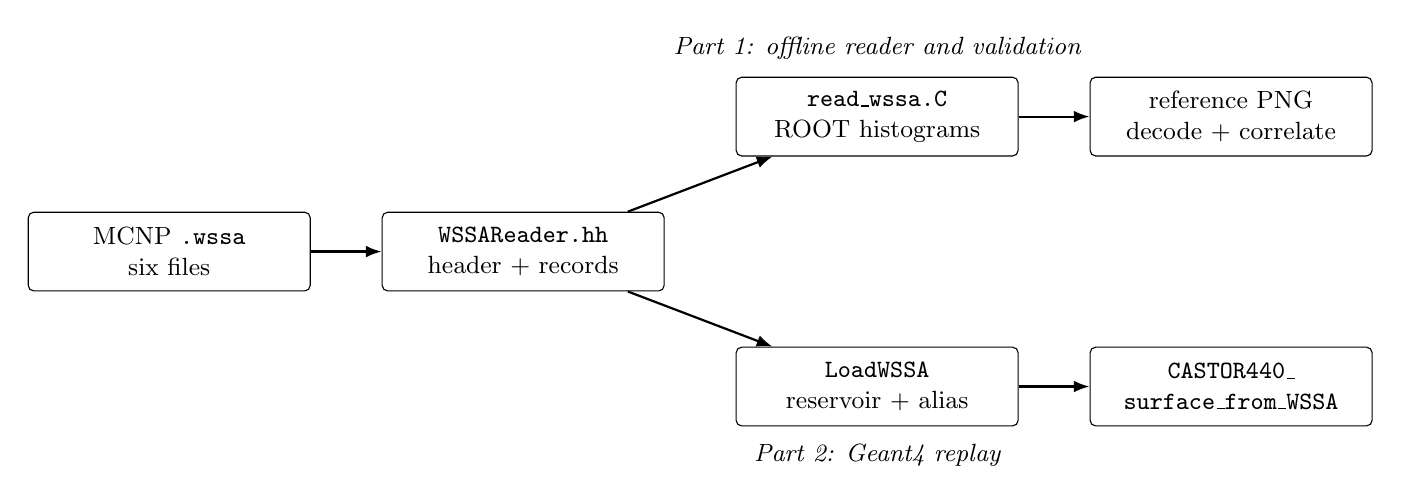
\begin{tikzpicture}[
  font=\small,
  box/.style={draw, rounded corners=2pt, align=center, inner sep=4pt,
              text width=3.3cm, minimum height=10mm},
  arr/.style={-{Latex[length=2mm]}, thick},
  node distance=7mm and 9mm
]
\node[box] (wssa) {MCNP \texttt{.wssa}\\six files};
\node[box, right=of wssa] (reader) {\texttt{WSSAReader.hh}\\header + records};
\node[box, above right=of reader] (root) {\texttt{read\_wssa.C}\\ROOT histograms};
\node[box, right=of root] (val) {reference PNG\\decode + correlate};
\node[box, below right=of reader] (load) {\texttt{LoadWSSA}\\reservoir + alias};
\node[box, right=of load] (g4) {\texttt{CASTOR440\_}\\\texttt{surface\_from\_WSSA}};
\draw[arr] (wssa) -- (reader);
\draw[arr] (reader) -- (root);
\draw[arr] (root) -- (val);
\draw[arr] (reader) -- (load);
\draw[arr] (load) -- (g4);
\node[above=1mm of root, font=\small\itshape]
  {Part 1: offline reader and validation};
\node[below=1mm of load, font=\small\itshape]
  {Part 2: Geant4 replay};
\end{tikzpicture}}
\caption{The shared binary parser and the two source branches.  Both branches
read the same particle records and use the same surface identifiers; only the
consumer differs.}
\label{fig:workflow}
\end{figure}

The report is not a detector-response validation and does not establish an
absolute dose calibration.  It establishes that the reader reproduces the
supplied angular and longitudinal structure, reports the absolute-scale
discrepancy under both stated WSSA normalizations, and shows that the Geant4
loader produces valid primaries.  Production yields still require a full
detector run.

% ---------------------------------------------------------------------------
\section{The WSSA file format}\label{sec:format}

\subsection{Record structure}

A \texttt{.wssa} file is a sequence of Fortran unformatted records.  Each record
is stored as
\begin{center}
\texttt{[4-byte length][payload][4-byte length]}
\end{center}
with little-endian byte order.  The prefix and trailer are equal; the reader
checks both and stops on a mismatch.  The payload size is the number of bytes
between the markers.  The header records and the particle stream are summarised
in Table~\ref{tab:format} and Figure~\ref{fig:format}.

\begin{table}[t]
\centering
\caption{Record layout used by all six files.  The record numbers are the
physical Fortran records, not particle indices.  The payload sizes are the
values read by \texttt{WSSAReader.hh}; a record may carry additional padding,
which is ignored.}
\label{tab:format}
\footnotesize
\begin{tabular}{@{}l l p{9.7cm}@{}}
\toprule
Record & Payload & Contents \\
\midrule
envelope & $4+n+4$ B & little-endian length markers; prefix and trailer must match \\
0 & 8 B & format identifier; the files contain \texttt{SF\_00001} \\
1 & $\ge$191 B & code name, version, build date, two date strings, \texttt{aid}, \texttt{knod} \\
2 & 32 B & \texttt{np} (i8), \texttt{nrsw} (i8), \texttt{nd} (i4), \texttt{njss} (i4), \texttt{nqsw} (i8) \\
3 & $\ge$12 B & \texttt{nilw} (i4), \texttt{mipt} (i4), \texttt{kq} (i4), padding \\
\texttt{njss} $\times$ surface & 20/24 B & \texttt{jss}, [\texttt{jsq}], \texttt{type}, \texttt{n}, \texttt{coeff}; 24 B when \texttt{kq}$\neq$0 \\
\texttt{nilw} $\times$ selected & variable & selected-surface records; none in these files \\
1 summary & variable & skipped by its recorded length \\
\texttt{nrsw} $\times$ particle & 88/56 B & 11 doubles, or 7 doubles for the symmetric variant; see text \\
\bottomrule
\end{tabular}
\end{table}

The header fields have the following meaning in this reader:
\begin{itemize}
  \item \texttt{np} and \texttt{nrsw} are 64-bit counts.  \texttt{nrsw} is the
        number of particle records, which is the count used by both consumers;
        \texttt{np} is retained as header metadata.
  \item \texttt{njss} is the number of surface records.  All six files have
        \texttt{njss}=4, \texttt{nilw}=0, \texttt{kq}=1, and \texttt{mipt}=37.
  \item The surface records describe three copies of the side cylinder and one
        top plane.  The side records have \texttt{jss}=11, 13, 15,
        \texttt{type}=15, and coefficient 17\,755.5625; the reader converts this
        to $R=1332.5$~mm.  The top record has \texttt{jss}=903,
        \texttt{type}=4, and coefficient 408.9, giving $z=4089$~mm.  There is no
        bottom-plane record.
\end{itemize}

\begin{figure}[t]
\centering
\resizebox{\linewidth}{!}{%
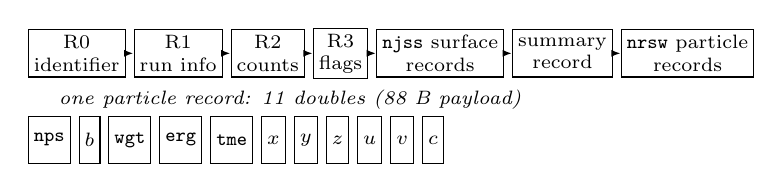
\begin{tikzpicture}[font=\scriptsize,
  rec/.style={draw, align=center, inner sep=2pt, minimum height=6mm},
  arr/.style={-{Latex[length=1.2mm]}, thick}]
\node[rec] (r0) {R0\\identifier};
\node[rec, right=1mm of r0] (r1) {R1\\run info};
\node[rec, right=1mm of r1] (r2) {R2\\counts};
\node[rec, right=1mm of r2] (r3) {R3\\flags};
\node[rec, right=1mm of r3] (rs) {\texttt{njss} surface\\records};
\node[rec, right=1mm of rs] (rm) {summary\\record};
\node[rec, right=1mm of rm] (rp) {\texttt{nrsw} particle\\records};
\draw[arr] (r0) -- (r1);
\draw[arr] (r1) -- (r2);
\draw[arr] (r2) -- (r3);
\draw[arr] (r3) -- (rs);
\draw[arr] (rs) -- (rm);
\draw[arr] (rm) -- (rp);

\node[rec, below=11mm of r0.west, anchor=west] (p0) {\texttt{nps}};
\node[rec, right=1mm of p0] (p1) {$b$};
\node[rec, right=1mm of p1] (p2) {\texttt{wgt}};
\node[rec, right=1mm of p2] (p3) {\texttt{erg}};
\node[rec, right=1mm of p3] (p4) {\texttt{tme}};
\node[rec, right=1mm of p4] (p5) {$x$};
\node[rec, right=1mm of p5] (p6) {$y$};
\node[rec, right=1mm of p6] (p7) {$z$};
\node[rec, right=1mm of p7] (p8) {$u$};
\node[rec, right=1mm of p8] (p9) {$v$};
\node[rec, right=1mm of p9] (p10) {$c$};
\node[above=2mm of p0, anchor=west, font=\scriptsize\itshape]
  {one particle record: 11 doubles (88 B payload)};
\end{tikzpicture}}
\caption{Top: the record sequence read before the particle stream.  Bottom: the
fields of one 88-byte particle record.  The 4-byte length markers are not drawn.
The reader also accepts a 56-byte symmetric record
(\texttt{nps}, $b$, \texttt{wgt}, \texttt{erg}, \texttt{tme}, $c_s$, $c$), but
the six files use the 88-byte form.}
\label{fig:format}
\end{figure}

\subsection{Particle records and units}

The 88-byte record contains eleven doubles in this order:
\begin{center}
\texttt{nps}, $b$, \texttt{wgt}, \texttt{erg}, \texttt{tme},
$x$, $y$, $z$, $u$, $v$, $c$.
\end{center}
The fields used by the source are:
\begin{itemize}
  \item \texttt{nps}: history or source-point number; the reader stores its
        absolute value.
  \item $b$: a sign carrier.  Only the sign is used, to reconstruct the third
        direction cosine
        \begin{equation}
          w = \operatorname{sgn}(b)\sqrt{\max(0,\,1-u^2-v^2)}.
        \end{equation}
        Both consumers then normalise $(u,v,w)$ to a unit vector.
  \item \texttt{wgt}: the MCNP statistical weight.
  \item \texttt{erg}: energy in MeV.
  \item $x,y,z$: position in cm, with $z=0$ at the floor.  The reader converts
        to mm by multiplying by ten; the Geant4 loader additionally shifts by
        $-H/2$ to the cask-centred frame.
  \item $u,v$: direction cosines in $x$ and $y$.
  \item $c$: surface label; its integer part is the surface identifier
        (\texttt{floor(c)}).  The fractional part is not used.
\end{itemize}
The 56-byte symmetric variant stores only seven doubles
(\texttt{nps}, $b$, \texttt{wgt}, \texttt{erg}, \texttt{tme}, $c_s$, $c$); it
has no explicit position or direction.  It is supported by the parser but does
not occur in these files.

\begin{table}[t]
\centering
\caption{The six source files and their reference images.  Sizes are decimal
GB; record counts are \texttt{nrsw} from the header.  The reference PNGs are the
maps used in Part~1.}
\label{tab:files}
\footnotesize
\setlength{\tabcolsep}{4pt}
\begin{tabular}{@{}l l r r l@{}}
\toprule
File & Particle & Size [GB] & Records & Reference PNG \\
\midrule
\texttt{Cask1\_gamma.wssa}    & $\gamma$ & 39.0 & \num{405872062} & \texttt{Cask1\_gamma.png} \\
\texttt{Cask1\_neutrons.wssa} & $n$ & 47.1 & \num{491077633} & \texttt{Cask1\_neutrons.png} \\
\texttt{Cask2\_gamma.wssa}    & $\gamma$ & 38.8 & \num{404226959} & \texttt{Cask2\_gamma.png} \\
\texttt{Cask2\_neutrons.wssa} & $n$ & 54.2 & \num{564324097} & \texttt{Cask2\_neutrons.png} \\
\texttt{Cask3\_gamma.wssa}    & $\gamma$ & 44.7 & \num{465772433} & \texttt{Cask3\_gamma.png} \\
\texttt{Cask3\_neutrons.wssa} & $n$ & 11.4 & \num{118939773} & \texttt{Cask3\_neutrons.png} \\
\bottomrule
\end{tabular}
\end{table}

\subsection{Geometry and frame}

The WSSA geometry and the Geant4 cask geometry are close but not identical
(Table~\ref{tab:geometry} and Figure~\ref{fig:geometry}).  The WSSA side
cylinder is at $R=1332.5$~mm; the Geant4 body is $R=1270$~mm and the fin tips
reach about 1330~mm.  The WSSA top plane is at $z=4089$~mm; the Geant4 cask is
4080~mm high.  The loader keeps the recorded crossing positions, so a top
record within 9~mm of the plane can start slightly above the Geant4 cap.  The
side surface is 2.5~mm outside the fin tips.

\begin{table}[t]
\centering
\caption{WSSA and Geant4 geometry.  The loader uses the cask height for the
$z$ shift; the radial and tolerance arguments are not used for WSSA because the
recorded positions are kept.}
\label{tab:geometry}
\footnotesize
\begin{tabular}{@{}>{\raggedright\arraybackslash}p{2.4cm}
                  >{\raggedright\arraybackslash}p{4.3cm}
                  >{\raggedright\arraybackslash}p{3.8cm}
                  >{\raggedright\arraybackslash}p{4.8cm}@{}}
\toprule
Quantity & WSSA & Geant4 & Consequence \\
\midrule
Side surface & \texttt{jss} 11/13/15, type 15, $R=1332.5$~mm
             & body $R=1270$~mm; fin tips $\approx1330$~mm
             & recorded side is 2.5~mm outside the fin tips \\
Top surface  & \texttt{jss} 903, type 4, $z=4089$~mm
             & cask height 4080~mm
             & top plane is 9~mm above the G4 cap \\
Bottom surface & none & bottom cap at $z=-2040$~mm
             & no bottom records; the loader would map them to surface~2 \\
Frame        & floor-based cm; $z=0$ at floor
             & cask-centred mm; $z=0$ at mid-height
             & loader uses $z_{\mathrm{mm}}-H/2$ \\
Particle     & 11 doubles (88~B)
             & \texttt{Crossing}: 8 floats and 2 ints (40~B)
             & direction normalised; weight kept in the alias table \\
\bottomrule
\end{tabular}
\end{table}

\begin{figure}[t]
\centering
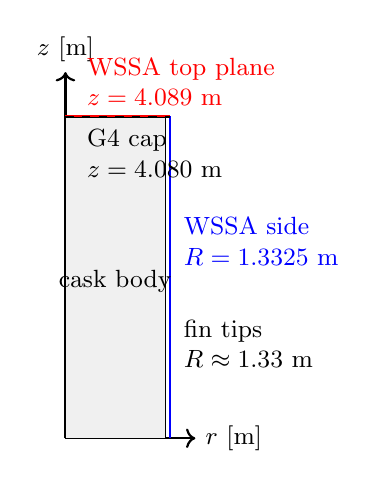
\begin{tikzpicture}[font=\small, scale=1.0]
\draw[->, thick] (0,0) -- (0,4.65) node[above] {$z$ [m]};
\draw[->, thick] (0,0) -- (1.65,0) node[right] {$r$ [m]};
\draw[fill=gray!12] (0,0) rectangle (1.27,4.08);
\draw[dashed] (1.33,0) -- (1.33,4.08);
\draw[blue, thick] (1.3325,0) -- (1.3325,4.089);
\draw[red, thick] (0,4.089) -- (1.3325,4.089);
\draw[dashed] (0,4.08) -- (1.3325,4.08);
\node at (0.63,2.0) {cask body};
\node[blue, align=left, anchor=west] at (1.38,2.5)
  {WSSA side\\$R=1.3325$~m};
\node[align=left, anchor=west] at (1.38,1.2)
  {fin tips\\$R\approx1.33$~m};
\node[red, align=left, anchor=south west] at (0.15,4.10)
  {WSSA top plane\\$z=4.089$~m};
\node[align=left, anchor=north west] at (0.15,4.04)
  {G4 cap\\$z=4.080$~m};
\end{tikzpicture}
\caption{Qualitative cross-section of the cask and the WSSA surfaces.  The
drawing is not to scale: the 2.5~mm side offset and the 9~mm top offset are
annotated but not visible at this scale.  The exact dimensions are in
Table~\ref{tab:geometry}.}
\label{fig:geometry}
\end{figure}

% ---------------------------------------------------------------------------
\section{Part 1: offline ROOT reader}\label{sec:part1}

\subsection{Parser and histograms}

\texttt{include/WSSAReader.hh} is a header-only, dependency-free parser.  It
opens the file, reads the header records, records the byte offset of the first
particle record, and exposes
\begin{itemize}
  \item \texttt{next(Record\&, err)} for a sequential pass, and
  \item \texttt{readAt(index, Record\&, err)} for O(1) random access.
\end{itemize}
Random access is valid because every particle record in these files has the
same on-disk size; \texttt{readAt} seeks to
\texttt{particleStart + index*particleRecordBytes}.  The reader validates the
prefix and trailer of every record and uses a 1~MiB buffer.  The parser is
shared with the Geant4 loader, so a format fix applies to both paths.

\texttt{scripts/wssa/read\_wssa.C} is the ROOT consumer.  It can sample random
indices or the first $N$ records, or stream every record with \texttt{N=0} and
\texttt{randomMode=false}; the validation uses the full stream.  It fills:
\begin{itemize}
  \item \texttt{hE}: 120 log-spaced energy bins from $10^{-12}$ to 30~MeV,
        weighted by \texttt{wgt};
  \item \texttt{hE\_linear}: 200 linear 20~keV bins from 0 to 4~MeV, filled for
        the gamma files only; it is used for the linear-axis gamma spectra;
  \item \texttt{hPhiZ}: the main $\varphi$--$z$ map; the full pass uses
        36 $\varphi$ bins and 41 $z$ bins over 0--4000~mm;
  \item \texttt{hPhiZ\_alt}: the same map in the complementary orientation;
  \item \texttt{hPhiZ\_0\_4000}: a presentation map with 36 $\varphi$ bins and
        80 $z$ bins over 0--4000~mm; it is not used for the final correlations;
  \item \texttt{hPhiZ\_fine}: a 360$\times$400 map for comparison with the
        reference images; the validation groups it 5$\times$5 onto the native
        72$\times$80 grid;
  \item \texttt{hPhiZ\_dose\_fine}: the same 360$\times$400 grid, filled with
        $w\,H^*(10)(E)$ instead of $w$; the validation groups it onto the
        reference grid in the same way;
  \item \texttt{hPhiZ\_side}, \texttt{hPhiZ\_top}, and
        \texttt{hPhiZ\_unknown}: maps split by the surface classification;
  \item \texttt{hPhi} and \texttt{hZ}: the one-dimensional projections.
\end{itemize}
The ROOT file also contains a \texttt{TNamed} called \texttt{wssa\_info} with
the input path, \texttt{nrsw}, \texttt{njss}, \texttt{kq}, the processed count,
the mode, the weighting flag, the summed weight, the side/top/unknown counts,
the energy-in-range count, the minimum and maximum energy and $z$, the
binning parameters, the inferred dose particle, and the summed $H^*(10)$ weight.

The angle conventions are:
\begin{align}
  \text{mode 0:}\quad & \varphi = \operatorname{atan2}(y,x),\\
  \text{mode 1:}\quad & \varphi = 90^\circ - \operatorname{atan2}(y,x),\\
  \text{mode 2:}\quad & \varphi = -\operatorname{atan2}(y,x),
\end{align}
each reduced to $[0,360^\circ)$.  Mode~1 is clockwise from $+y$; mode~0 is
counter-clockwise from $+x$; mode~2 is clockwise from $+x$.  The default and
the mode used for the full validation pass is mode~1, because the supplied
reference images use a clockwise angle.

The surface classification in the ROOT reader is geometric.  For a record with
surface identifier \texttt{id}, the reader looks up the header coefficient
\texttt{coeff} and computes
\[
  d_{\text{cyl}} = \left|\sqrt{\texttt{coeff}} - \sqrt{x^2+y^2}\right|,
  \qquad
  d_{\text{plane}} = \left|\texttt{coeff} - z\right|,
\]
with both distances in cm.  A record is on the side if
$d_{\text{cyl}}<0.5$~cm and $d_{\text{cyl}}<d_{\text{plane}}$; it is on the top
if $d_{\text{plane}}<0.5$~cm; otherwise it is unknown.  In the six full passes
the unknown count is zero.

\subsection{Full-file pass and integral checks}

The validation pass uses
\texttt{N=0}, \texttt{randomMode=false}, \texttt{phiMode=1},
\texttt{weighted=true}, 36 $\varphi$ bins, 41 $z$ bins, $z_{\max}=4000$~mm,
120 energy bins, $E_{\min}=10^{-12}$~MeV, $E_{\max}=30$~MeV, seed 12345, and
the dose-particle tag inferred from the file name (\texttt{gamma} or
\texttt{neutron}).
It reads every record exactly once and fills the histograms in place; the
reader does not store the full record vector.  The histograms are filled with
the record weight, so the map is the full-file sum of weights, not a sample
sum.

\begin{table}[t]
\centering
\caption{Full-file pass over all six WSSA files.  Records are the header
\texttt{nrsw}; side and top are the geometric classification counts from
\texttt{read\_wssa.C}; unknown is zero in every file.  The energy range is the
range of all records.  The last column is the full-file sum of weights divided
by the header $|np|$.  The raw sum is the sum of weights; WTI's stated
normalization would make it a crossing rate, but the scale test in
Section~\ref{sec:absolute_scale} does not support that interpretation.  The
per-history column is used for the PNG comparison; the raw sum is reported in
Table~\ref{tab:absolute_scale}.  For
the neutron files the last column is the total of neutrons and photons; the
type-resolved values are in Table~\ref{tab:p1_wssa}.  Every record fell inside
the histogram range.}
\label{tab:samples}
\footnotesize
\begin{tabular}{@{}l r r r r l r@{}}
\toprule
File & Records & Side & Top & Unknown & Energy [MeV] & Sum/$|np|$ [per history] \\
\midrule
\texttt{Cask1\_gamma}    & \num{405872062} & \num{405840179} & \num{31883}
  & 0 & $1.02\times10^{-3}$--3.65 & $2.983\times10^{7}$ \\
\texttt{Cask1\_neutrons} & \num{491077633} & \num{449256321} & \num{41821312}
  & 0 & $2.44\times10^{-10}$--19.89 & $1.889\times10^{7}$ \\
\texttt{Cask2\_gamma}    & \num{404226959} & \num{404196984} & \num{29975}
  & 0 & $1.02\times10^{-3}$--3.85 & $1.172\times10^{7}$ \\
\texttt{Cask2\_neutrons} & \num{564324097} & \num{535715406} & \num{28608691}
  & 0 & $4.70\times10^{-11}$--20.44 & $1.500\times10^{6}$ \\
\texttt{Cask3\_gamma}    & \num{465772433} & \num{465652828} & \num{119605}
  & 0 & $1.01\times10^{-3}$--3.95 & $4.346\times10^{6}$ \\
\texttt{Cask3\_neutrons} & \num{118939773} & \num{85928383} & \num{33011390}
  & 0 & $1.90\times10^{-10}$--19.55 & $1.178\times10^{7}$ \\
\bottomrule
\end{tabular}
\end{table}

The header $|np|$ is $10^{8}$ for all three neutron files, $10^{11}$ for the
Cask~1 and Cask~2 gamma files, and $5\times10^{11}$ for the Cask~3 gamma file.
The last record's history number equals $|np|$ in every file, so the files are
complete and the divisor is the number of MCNP source histories.

The energy histogram integral equals the sum of the filled weights in all six
full passes.  This checks the weight handling and the log-bin edges.  The top
fraction is largest for Cask~3 neutrons (33\,011\,390 of 118\,939\,773, or
27.75\%); the other files range from 0.007\% to 8.5\%.  The top records lie at
$z=4089$~mm, outside the 0--4000~mm maps used for the image comparison; the
side/top counts are tallies, not map entries.

A separate sequential check on 2\,000 Cask~3 neutron records shows consecutive
bit-identical groups.  The groups have multiplicities up to 16; the full Cask~3
gamma pass contains groups up to multiplicity 20.  These are MCNP
importance-splitting copies: the same history crosses the surface more than
once and receives a different weight.  The reader keeps them; the Geant4 alias
table samples them in proportion to their weights.  No de-duplication is
applied.

\subsection{Reference-map decoding}

The reference PNGs are 1600$\times$800 images with the same layout: a plot frame
and a vertical colour bar.  For these six images the frame is at
$x=177$--$1346$, $y=69$--$653$, and the colour bar is at $x=1375$--$1433$.
The decoder is the ROOT macro \texttt{scripts/wssa/validate\_wssa\_root.C}.
It reads the PNG with \texttt{TASImage::GetArgbArray}; \texttt{GetPixels}
returns zero for these images.  It then:
\begin{enumerate}
  \item detects the frame and colour bar from the long dark lines;
  \item samples the centre of the colour bar from top to bottom and assigns
        value 1 to the top (red) end and 0 to the bottom (blue) end;
  \item builds a nearest-colour lookup from the bar samples and maps every
        heat-map pixel to that ordinal value;
  \item masks white pixels, black pixels, and colours farther than 35 RGB units
        from the bar;
  \item maps the remaining pixels to $\varphi\in[0,360^\circ)$ from left to
        right and $z\in[0,4000]$~mm from bottom to top;
  \item averages the pixels in the same bins as the ROOT histogram and computes
        the Pearson correlation of the binned maps and of the two profiles.
\end{enumerate}
The decoded value is an ordinal colour-bar coordinate.  For display, each
reference map is scaled by the maximum printed on its own colour bar: 60, 5, 6,
1.4, 35, and 2.5~$\mu$Sv\,h$^{-1}$ for Cask~1 neutrons, Cask~1 gamma, Cask~2
neutrons, Cask~2 gamma, Cask~3 neutrons, and Cask~3 gamma.

The WSSA weights are MCNP statistical weights.  WTI states that the sum over
the complete file is the total number of particles crossing the tally surface
per second.  If that statement is applied literally, the raw weights are
particles per second.  The direct check in Section~\ref{sec:absolute_scale}
does not support that reading, so the raw sum is retained as the documented
WTI convention and as the default replay mode, not as a validated absolute
calibration.  The header also provides the number of source histories $|np|$;
dividing the raw sum by $|np|$ gives crossings per source history.  A single
global factor cannot convert either map to dose rate because the flux-to-dose
coefficient depends on particle energy and the spectrum varies across the map.  The reader therefore fills a second map with an
energy-dependent coefficient per record,
\[
  h^{H^*(10)}_{\varphi z}
  = \sum_{i\in\text{bin}} w_i\,H^*(10)(E_i).
\]
Under the stated absolute interpretation, the corresponding dose rate is
\[
  \dot H_{\varphi z}
  = \frac{h^{H^*(10)}_{\varphi z}}{A_{\varphi z}}
    \times \frac{3600}{10^{6}}~\mu\text{Sv\,h}^{-1},
\]
where \(A_{\varphi z}\) is the surface area of the bin in cm\(^2\), 3600 is
s\,h\(^{-1}\), and \(10^{6}\) is pSv\,$\mu$Sv\(^{-1}\).  The WSSA header
gives \(|np|\); the reference tally area and estimator are not in the file.
The reader normalises the sum-of-weights shape maps to their own maxima for
display.  It draws the $H^*(10)$ maps per source history, dividing by $|np|$
and by the bin area, so their colour bars are in $\mu$Sv\,h$^{-1}$ and can be
compared directly with the reference PNGs.  No per-maximum normalisation is
applied to the $H^*(10)$ maps; the raw-sum absolute scale is reported separately
in Section~\ref{sec:absolute_scale}.
The coefficient arrays in \texttt{ICRP74H10.hh} contain the ICRP~74/ICRU~57
ambient dose equivalent $H^*(10)$ data\footnote{ICRP Publication 74,
\emph{Conversion Coefficients for Use in Radiological Protection against
External Radiation} (1996); ICRU Report 57, \emph{Conversion Coefficients for
Use in Radiological Protection against External Radiation} (1998).  The
tabulated values are those distributed with the OpenMC data package.}: 25
photon points from 0.01 to 10~MeV and 47 neutron points from $10^{-9}$ to
20~MeV, interpolated log--log and clamped at the endpoints.  Table~\ref{tab:dose_coeff}
shows a few of those points; it is not the full coefficient set.
$H^*(10)$ is the operational ambient dose equivalent appropriate to an area
dose-rate map.  ``Ambient dose'' here is not a separate conversion table: it is
the operational quantity \(H^*(10)\) evaluated at 10~mm depth in the ICRU
sphere.  An effective-dose conversion would need a stated phantom and
irradiation geometry, which the supplied images do not provide.  The working assumption is therefore
that the printed \texttt{gDL} and \texttt{nDL} scales are $H^*(10)$ dose rates.
For orientation, Table~\ref{tab:dose_coeff} lists selected \(H^*(10)\),
effective-dose AP, and effective-dose ISO coefficients.  The effective-dose
coefficients depend on the irradiation geometry; the values shown are for a
phantom facing the source (AP) and for isotropic incidence (ISO).  \(H^*(10)\)
is generally the larger quantity at low photon energies and for neutrons near
1~MeV, while the AP effective dose exceeds \(H^*(10)\) for neutrons near
10~MeV.  The ratio is therefore energy-dependent even when the reference is a
dose quantity, which is why a single global factor cannot map particle/s to
dose.

\begin{table}[H]
\centering
\caption{Selected ICRP~74 conversion coefficients in
pSv\,cm\(^2\).  The \(H^*(10)\) values are the ones used in this report; the
effective-dose AP and ISO columns are shown only to illustrate the
quantity and geometry dependence.  The table is not used to produce the
reader maps.}
\label{tab:dose_coeff}
\footnotesize
\begin{tabular}{@{}l r r r r@{}}
\toprule
Particle & \(E\) [MeV] & \(H^*(10)\) & \(E_{\rm AP}\) & \(E_{\rm ISO}\) \\
\midrule
Photon & 0.1 & 0.61 & 0.517 & 0.278 \\
Photon & 1 & 5.20 & 4.48 & 3.21 \\
Photon & 10 & 25.6 & 23.8 & 20.8 \\
\midrule
Neutron & \(10^{-8}\) & 9.0 & 6.55 & 2.89 \\
Neutron & \(10^{-2}\) & 10.5 & 18.3 & 7.70 \\
Neutron & 1 & 416 & 282 & 116 \\
Neutron & 10 & 440 & 499 & 309 \\
\bottomrule
\end{tabular}
\end{table}
\subsection{Absolute-scale diagnostic}\label{sec:absolute_scale}

The diagnostic uses the existing full-statistics $h^{H^*(10)}_{\varphi z}$ map
for the F1 estimator and a 10-million-record sequential sample for the F2
estimator.  F1 is the surface-crossing sum, with one contribution per record;
F2 is the same sum divided by $|\mu|$, where $\mu$ is the direction cosine to
the surface normal, so it is a crossing-to-fluence estimator.  The native side
bin has
$A_{\varphi z}=R\,\Delta\varphi\,\Delta z=58.141$~cm$^2$.  The F2 value in
Table~\ref{tab:absolute_scale} is estimated at the hot bin of the full F1 map
from the local F2/F1 ratio in the sample; it is not a sample maximum.

\begin{table}[H]
\centering
\caption{Absolute-scale diagnostic at the native 72$\times$80 side bins.
The PNG maximum is the value printed on each colour bar.  The raw ratio uses
the full-statistics F1 map and the stated area.  The F1 and F2 per-history
values use the full F1 map and the local F2/F1 ratio from the 10-million-record
sample.  The F2 estimator is the same dose weight divided by $|\mu|$; it is not
a better match for the neutron files.}
\label{tab:absolute_scale}
\footnotesize
\begin{tabular}{@{}l r r r r r r@{}}
\toprule
File & $|np|$ & PNG max & raw/PNG & F1/$|np|$ & F1/$|np|$/PNG & F2/$|np|$/PNG \\
     &        & [$\mu$Sv\,h$^{-1}$] & & [$\mu$Sv\,h$^{-1}$] & & \\
\midrule
C1 n & $10^{8}$  & 60  & $1.31\times10^{8}$  & 78.84  & 1.31 & 1.87 \\
C1 g & $10^{11}$ & 5   & $5.36\times10^{10}$ & 2.682  & 0.54 & 0.71 \\
C2 n & $10^{8}$  & 6   & $1.30\times10^{8}$  & 7.827  & 1.30 & 1.79 \\
C2 g & $10^{11}$ & 1.4 & $7.84\times10^{10}$ & 1.097  & 0.78 & 0.99 \\
C3 n & $10^{8}$  & 35  & $1.44\times10^{8}$  & 50.31  & 1.44 & 2.07 \\
C3 g & $5\times10^{11}$ & 2.5 & $2.14\times10^{11}$ & 1.072 & 0.43 & 0.54 \\
\bottomrule
\end{tabular}
\end{table}

The raw sum-of-weights map is $1.3\times10^{8}$--$2.1\times10^{11}$ times the
PNG colour bar.  This cannot be the same surface with the stated bin area.  The
per-history F1 map is within a factor 0.43--1.44 of the PNG maximum; the F2
variant is within 0.54--2.07 and is worse for all three neutron files.  The
per-history F1 map is therefore the only same-surface interpretation close to
the supplied scale, but it is an empirical comparison, not a calibration.  The
residual factor is not removed by the area or the $|\mu|$ conversion and is
attributed to the unknown reference estimator, dose quantity, and colour-bar
decoding.  The PNG is used as a reader-correctness and per-history reference,
not as an absolute inventory-rate calibration.  The Geant4 sampler supports
both interpretations: the default WSSA mode follows WTI's stated absolute
convention, and \texttt{/dcs-monitor/surf/wssaAbsoluteWeight false} selects
$N=T\,S\,\sum w/|np|$ for the per-history comparison.  Neither mode is
validated as an absolute source rate by this report.

All 72$\times$80 and 36$\times$41 reference bins are finite in all six images,
and the median nearest-colour distance is zero.  The supplied PNGs are
reproduced unchanged in Figure~\ref{fig:orig}; the digitised reference maps are
shown in Figure~\ref{fig:reference_all} and in the Cask~3 comparison of
Figure~\ref{fig:maps}.

The reference images are digitised directly on their native 72$\times$80 grid.
The 2D score groups the reader's 360$\times$400 \texttt{hPhiZ\_fine} map
5$\times$5 onto the same cell edges; no interpolation is used.  The
$\varphi$-profile score is the mean over the 80 $z$ bins of the 72$\times$80
map, and the $z$-profile score is the mean over the 72 $\varphi$ bins.  The
36$\times$41 \texttt{hPhiZ} and \texttt{hPhiZ\_alt} pair is retained only for
the mode-0 orientation check; the reference is digitised on the same
36$\times$41 grid for that comparison.

\begin{figure}[t]
\centering
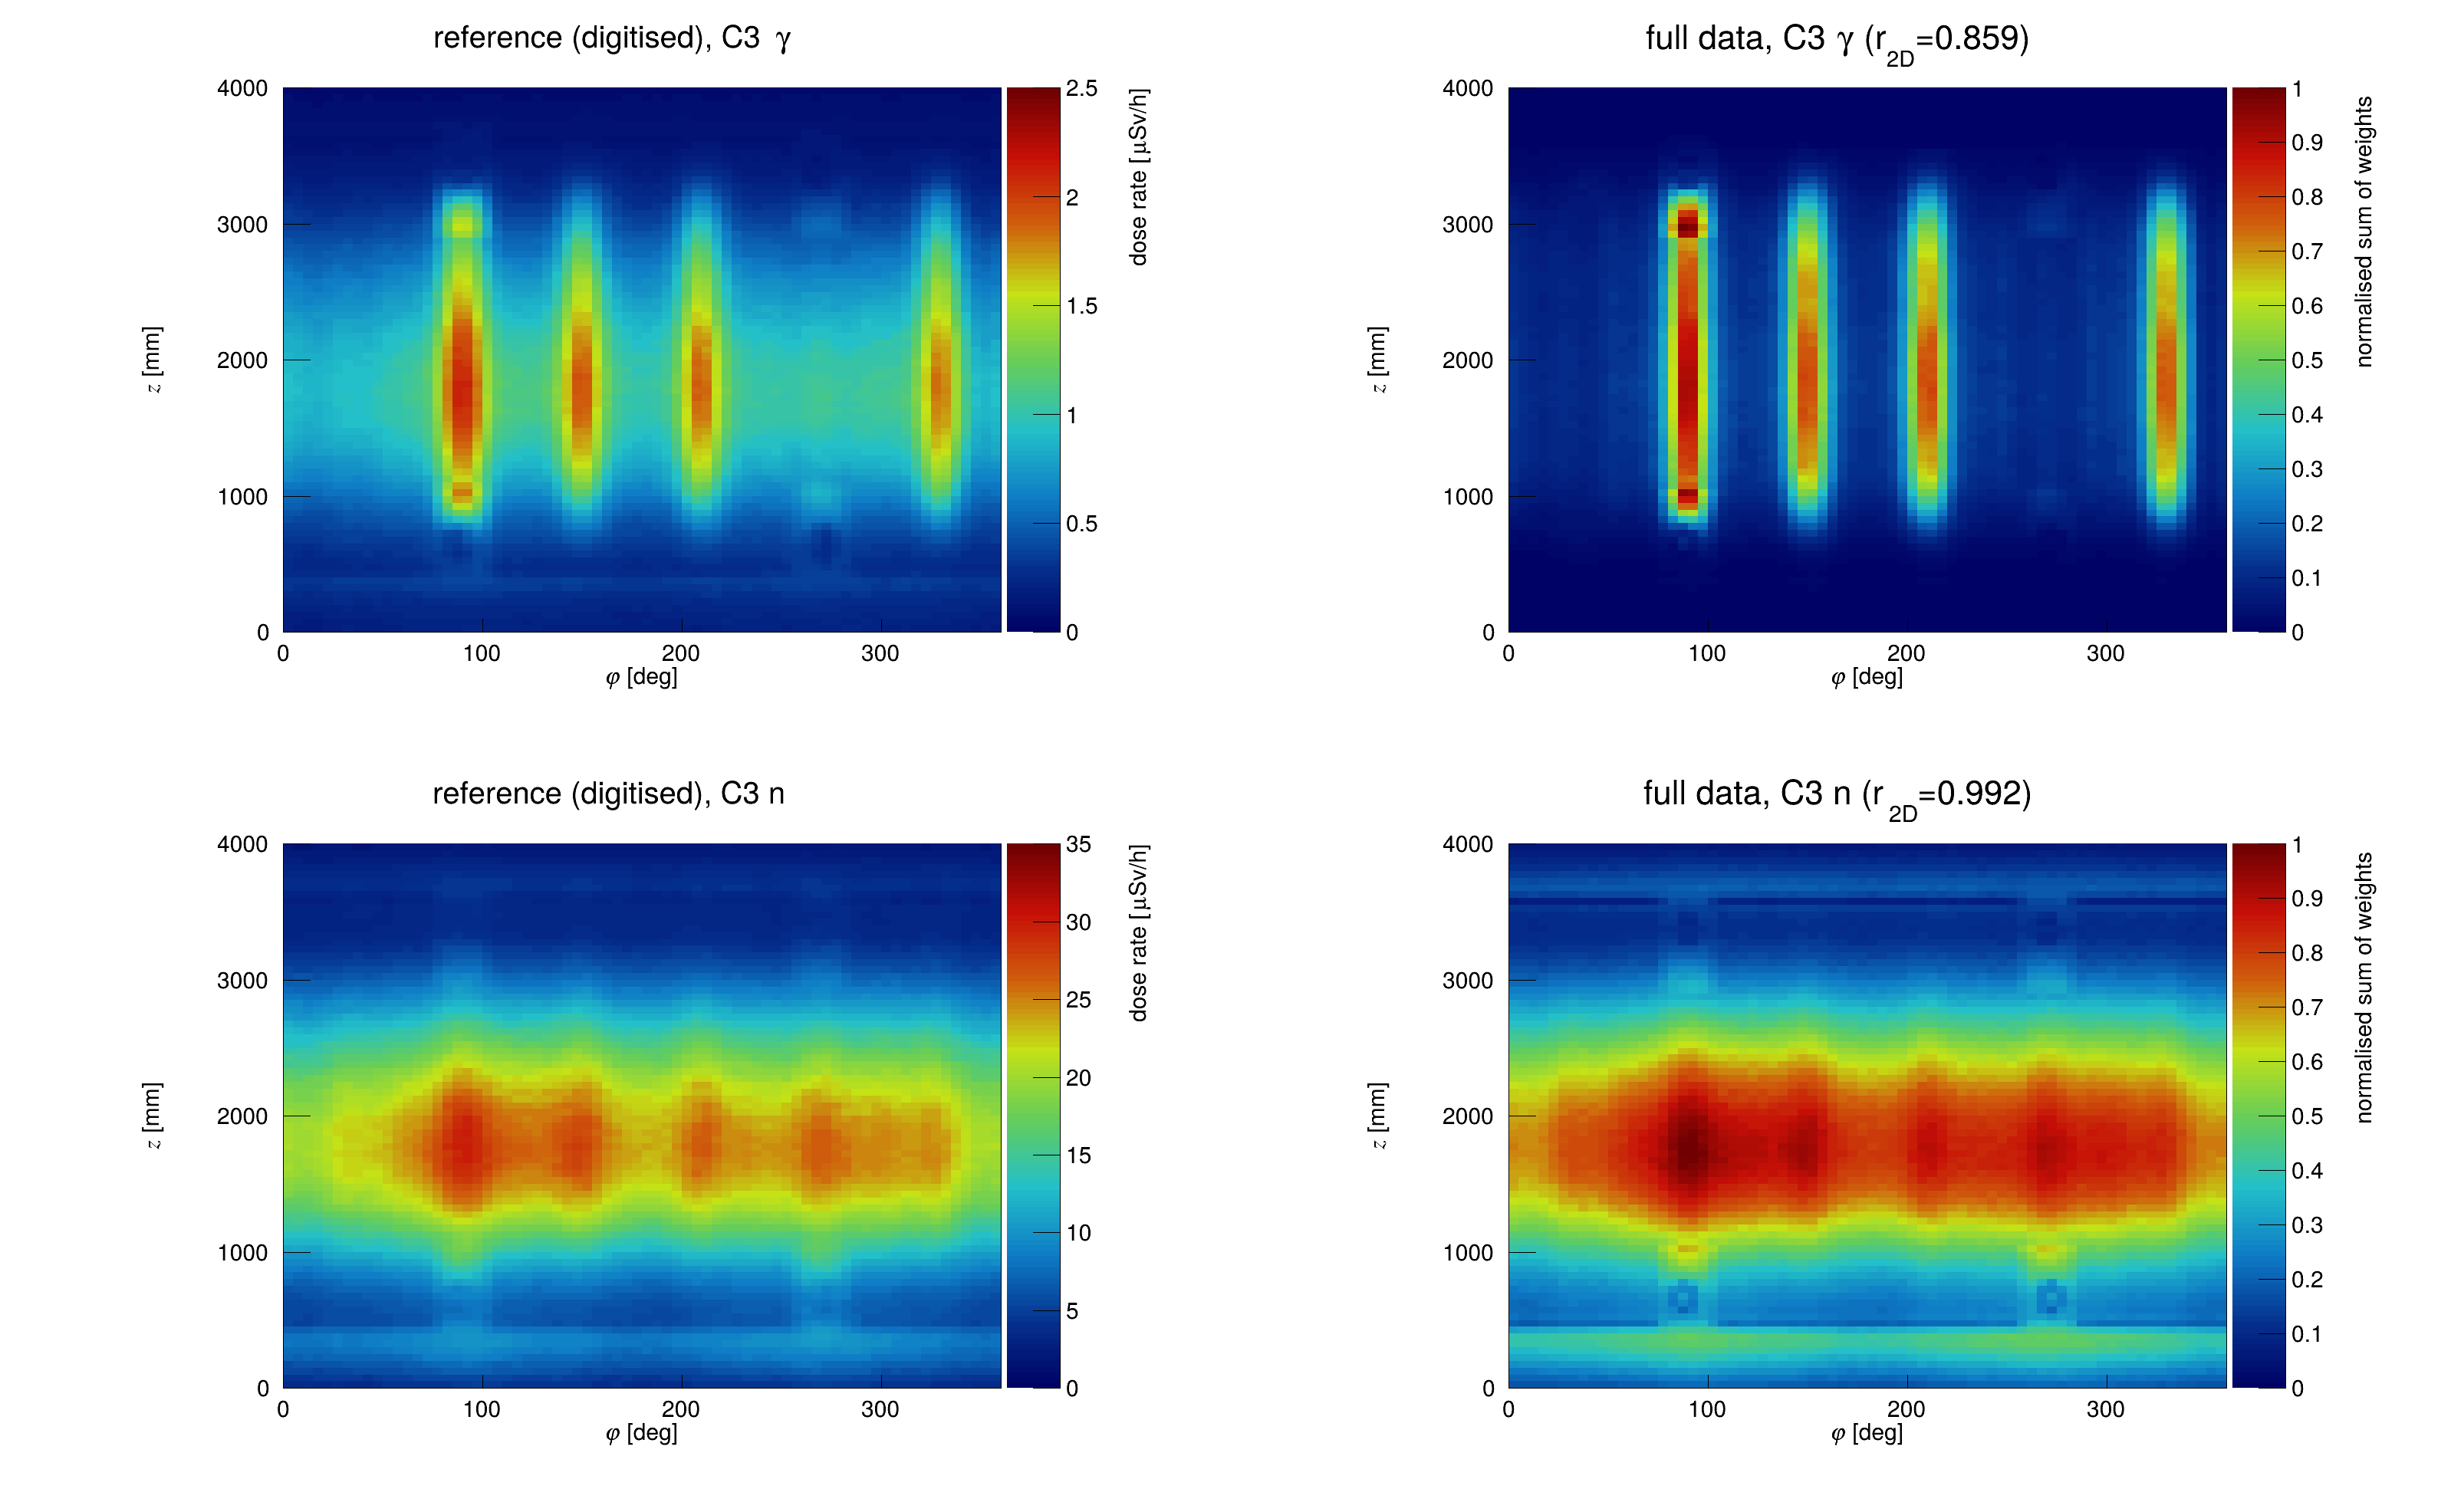
\includegraphics[width=\linewidth]{fig_maps_Cask3.png}
\caption{Cask~3 maps from the full-file pass.  The left column is the digitised
reference and the right column is the full reader; the top row is gamma and
the bottom row is neutrons: (a) reference gamma, (b) reader gamma, (c)
reference neutrons, (d) reader neutrons.  The reference panels use the dose-rate scale
from their own colour bars ($\mu$Sv\,h$^{-1}$); the reader panels are
normalised sums of weights with separate 0--1 colour bars.  The maps are drawn
on the reference's native 72$\times$80 grid ($5^\circ\times50$~mm); the
correlation in a reader title is the 72$\times$80 map correlation: 0.859 for
gamma and 0.992 for neutrons.  The reader panels use mode~1 (clockwise from
$+y$).}
\label{fig:maps}
\end{figure}

\subsection{Results}

Table~\ref{tab:validation} lists the correlations for all six files.
Figure~\ref{fig:maps} shows the Cask~3 maps, Figures~\ref{fig:zprofiles}
and~\ref{fig:phiprofiles} show all six profiles, and Figure~\ref{fig:scores}
summarises the scores.

\begin{table}[H]
\centering
\caption{Pearson correlations between the decoded reference image and the
full-file reader maps.  The 2D column is the native 72$\times$80 map over
0--4000~mm; the $\varphi$ mode~1 column is the 72$\times$80 map; the
$\varphi$ mode~0 column is the 36$\times$41 orientation grid; the $z$ column is
the 72$\times$80 map.  Peaks are image/reader.  The superscript marks the Cask~1
gamma double lobe discussed below.}
\label{tab:validation}
\footnotesize
\begin{tabular}{@{}l r r r r l l@{}}
\toprule
File & 2D & $\varphi$ mode 1 & $\varphi$ mode 0 & $z$
     & $z$ peak [mm] & $\varphi$ peak [deg] \\
\midrule
\texttt{Cask1\_gamma}    & 0.989 & 0.996 & 0.899 & 0.994 & 1825/1825 & 82.5/82.5\textsuperscript{a} \\
\texttt{Cask1\_neutrons} & 0.998 & 0.981 & 0.612 & 0.999 & 1825/1825 & 262.5/262.5 \\
\texttt{Cask2\_gamma}    & 0.998 & 0.994 & 0.426 & 0.999 & 1775/1725 & 97.5/102.5 \\
\texttt{Cask2\_neutrons} & 0.998 & 0.971 & $-0.393$ & 0.999 & 1775/1775 & 267.5/272.5 \\
\texttt{Cask3\_gamma}    & 0.859 & 0.981 & $-0.394$ & 0.952 & 1775/1825 & 92.5/87.5 \\
\texttt{Cask3\_neutrons} & 0.992 & 0.995 & $-0.729$ & 0.992 & 1775/1725 & 92.5/92.5 \\
\bottomrule
\end{tabular}
\par\smallskip
\begin{minipage}{0.96\linewidth}
\footnotesize
\textsuperscript{a}The Cask~1 gamma map has two near-equal maxima.  The image
values are 1.0000 at $82.5^\circ$ and 0.9997 at $262.5^\circ$; the reader values
are 1.0000 at $82.5^\circ$ and 0.9990 at $262.5^\circ$.  The table lists the
global maximum.  The $\varphi$-profile correlation is 0.996, so the double lobe
is reproduced, with both maxima in the same $5^\circ$ bins.
\end{minipage}
\end{table}

The main observations are:
{\small
\begin{itemize}
  \item \textbf{The 2D maps agree.}  Five of the six particle/s
        correlations are at least 0.989.  Cask~3 gamma is the lowest at 0.859;
        its $\varphi$ and $z$ profiles are 0.981 and 0.952.  This is a contrast
        difference, not a peak-position error.  The peaks agree within one bin:
        the image and reader $\varphi$ peaks are 92.5$^\circ$ and 87.5$^\circ$,
        and the $z$ peaks are 1775~mm and 1825~mm.  For the unweighted map, no
        one-bin shift improves the 2D score by more than 0.004; the best shift
        is 50~mm and raises it only from 0.859 to 0.863, while a one-bin
        $\varphi$ shift lowers it.  The reference has a higher smooth baseline
        between the four $\varphi$ bands and above and below the axial ends;
        the reader falls closer to zero there and is sharper in the band cores
        (Figure~\ref{fig:maps}c,d).  In the valleys the reference $\varphi$
        profile is 0.407--0.510 and the reader is 0.106--0.147; at 375~mm the
        $z$ profile is 0.282 for the reference and 0.027 for the reader.  The
        projections average over the other coordinate and stay high; the 2D
        score samples every cell.  A high-pass test that subtracts a
        Gaussian-smoothed component ($\sigma=2$ bins,
        $10^\circ\times100$~mm) from both maps raises the unweighted 2D score
        to 0.978, so the fine structure agrees and the smooth baseline is the
        remaining difference.  None of the other five maps shows this increase;
        each has a lower high-pass score than raw score.  Grouping to
        36$\times$80 changes the score by less than 0.003, and a constant
        scaling does not change a Pearson correlation, so binning and
        maximum-scaling are excluded.
        Applying the $H^*(10)$ coefficients per record raises the Cask~3 gamma
        score only from 0.859 to 0.867; its $\varphi$ and $z$ profiles become
        0.982 and 0.953, and the high-pass score remains 0.976.  The smooth
        baseline is still absent from the $H^*(10)$ map
        (Figure~\ref{fig:maps_dose}c,d).  The residual is therefore not
        explained by the energy dependence of the flux-to-dose coefficient
        alone.  It is consistent with a difference in the reference tally
        definition or normalisation, or with a contribution that is not present
        in the surface-crossing record set; the supplied images and WSSA files
        do not contain the information needed to separate these possibilities.
  \item \textbf{Mode~1 is the reference convention.}  The
        $\varphi$-profile correlation is higher in mode~1 for all six files.
        For Cask~1 neutrons the $\varphi$ profile is 0.981 in mode~1 and 0.612
        in mode~0; the projection is the more sensitive orientation test.
  \item \textbf{The Cask~1 gamma double lobe is reproduced.}  The image and the
        reader both have maxima at $82.5^\circ$ and $262.5^\circ$.  The global
        maximum is $82.5^\circ$ in both, and the second maximum is 0.9997 in
        the image and 0.9990 in the reader; the profile correlation 0.996
        shows that the two-lobe shape agrees.
  \item \textbf{The gamma $z$ peak is close to the image.}  The Cask~1 gamma
        peak matches at 1825~mm; the Cask~2 gamma reader peak is 50~mm lower,
        and the Cask~3 gamma reader peak is 50~mm higher.  The particle/s $z$
        correlations are 0.994, 0.999, and 0.952; the $H^*(10)$ values are
        0.995, 0.999, and 0.953.  The $H^*(10)$ weighting moves the Cask~1
        gamma peak from 1825 to 1875~mm and leaves the other two within one bin,
        so the peak position is sensitive to the weighting while the profile
        correlation remains high.  The neutron peaks agree within 50~mm.
  \item \textbf{The comparison is morphological.}  The colour-bar decoding is
        ordinal; the absolute dose scale is used only for the reference display
        and not in the correlation.  The top 89~mm of the WSSA source is outside
        the 0--4000~mm maps.  The scores are a consistency check, not a
        calibration.
\end{itemize}
}

\begin{figure}[t]
\centering
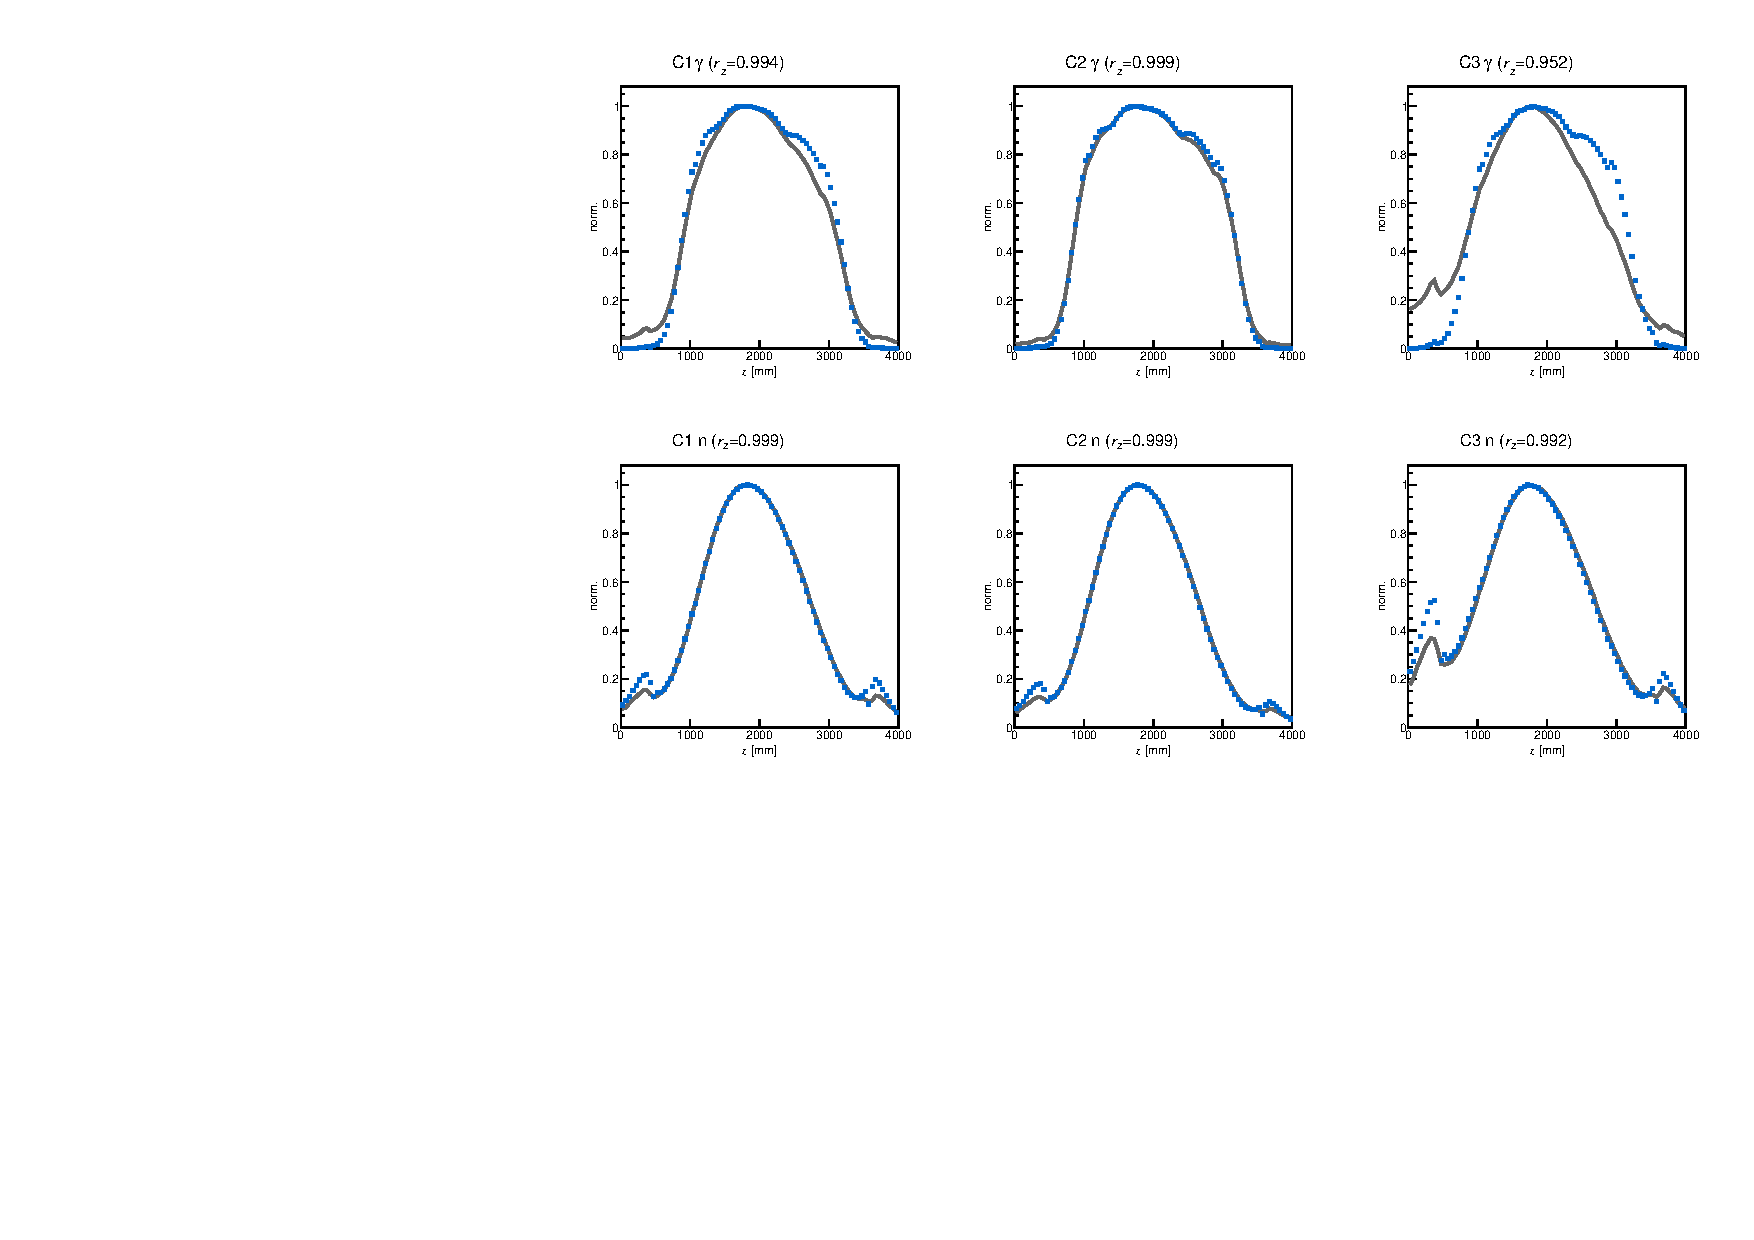
\includegraphics[width=\linewidth]{fig_validation_z_profiles_all.pdf}
\caption{$z$ profiles for all six full-file maps.  Columns are Cask~1, 2, and
3 from left to right; the top row is gamma and the bottom row is neutrons.
Each panel compares the digitised reference image (grey line) with the full
reader map (blue markers), normalised to its maximum.  The title gives the
$z$-profile correlation.  The reference is a dose-rate map and the reader is a
weight sum; the weight sum divided by the header $|np|$ is a per-history
multiplicity.  The raw sum is the sum of weights; its absolute interpretation is
tested in Section~\ref{sec:absolute_scale}.  The profiles test the vertical
structure, not the absolute normalisation.}
\label{fig:zprofiles}
\end{figure}

\begin{figure}[t]
\centering
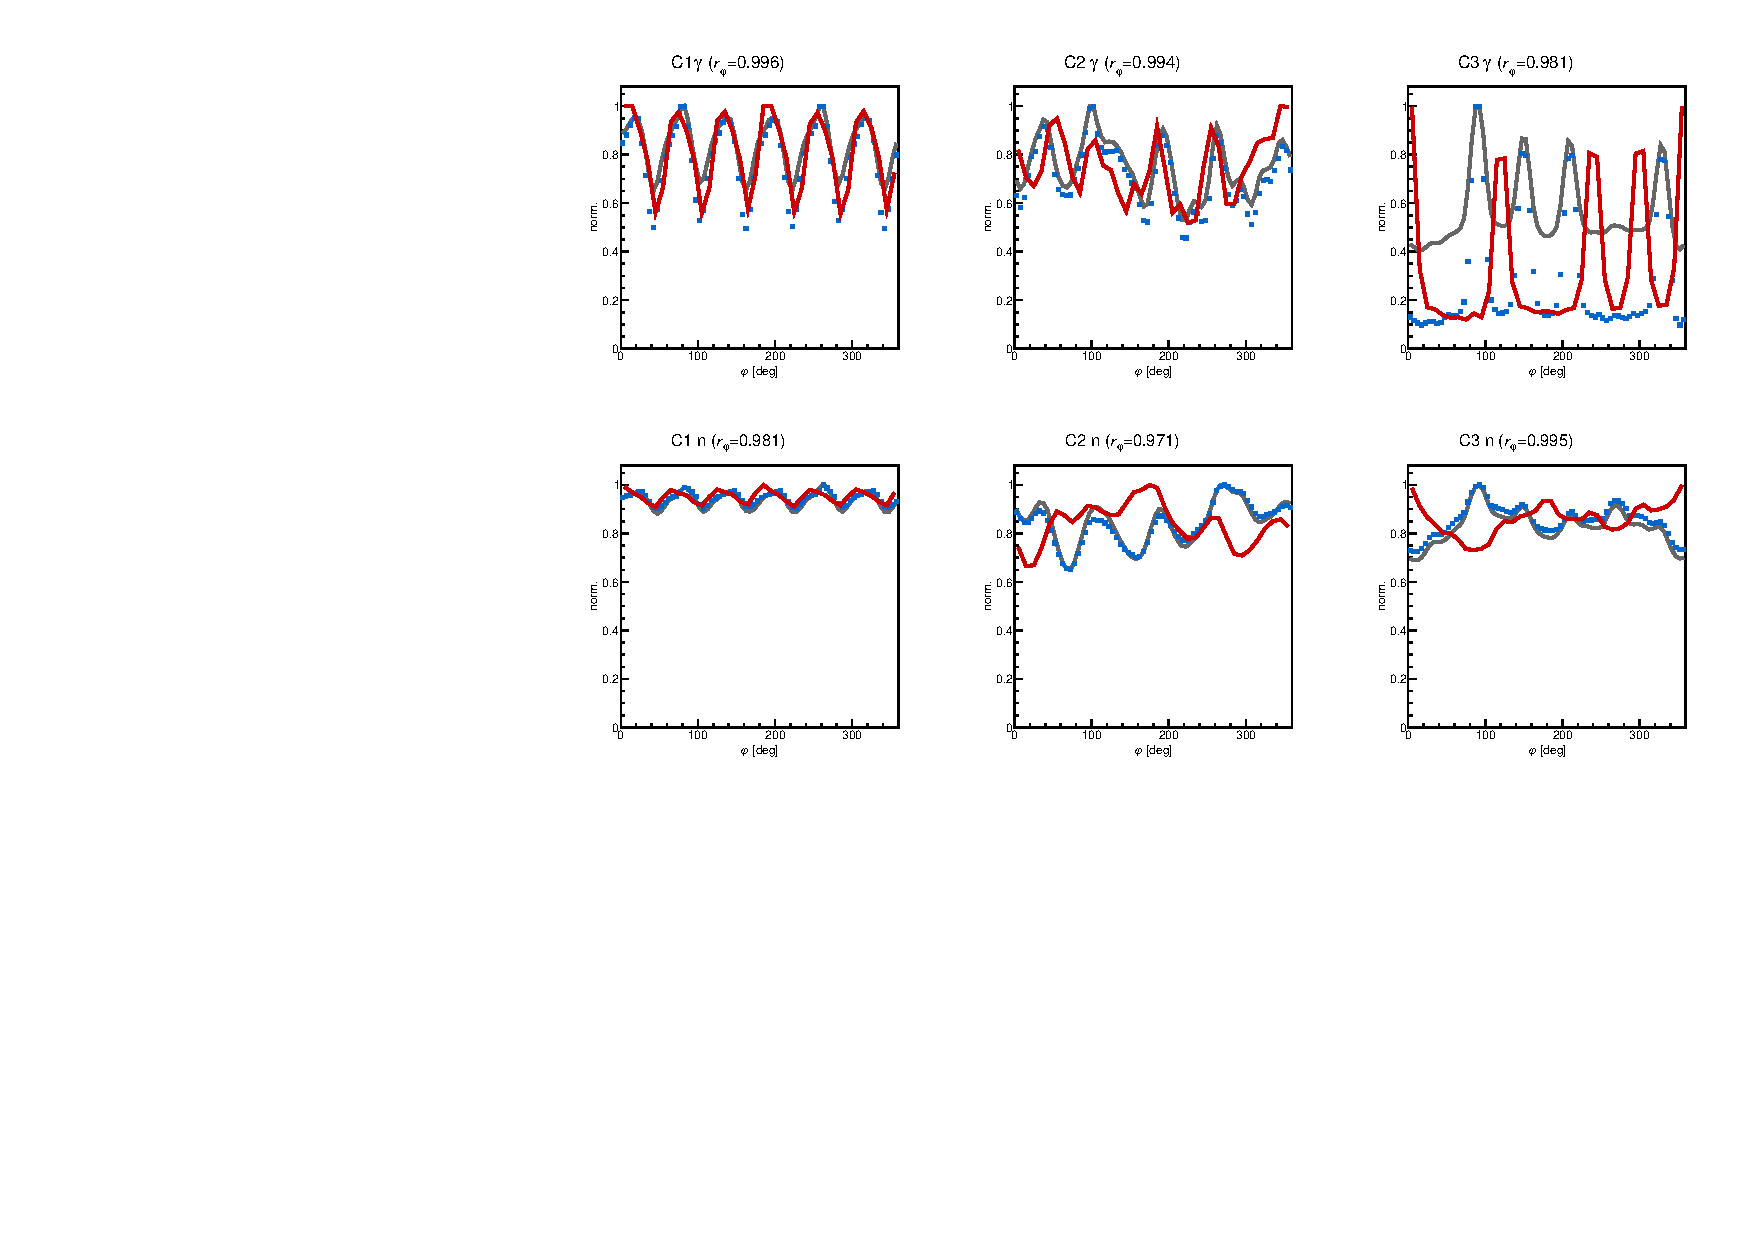
\includegraphics[width=\linewidth]{fig_validation_phi_profiles_all.pdf}
\caption{$\varphi$ profiles for all six full-file maps.  Columns are Cask~1,
2, and 3 from left to right; the top row is gamma and the bottom row is
neutrons.  Each panel compares the digitised reference image (grey line), the
reader map in mode~1 (clockwise from $+y$, blue markers), and the reader map in
mode~0 (counter-clockwise from $+x$, red line).  Profiles are normalised to
their maxima.  The title gives the mode~1 correlation.}
\label{fig:phiprofiles}
\end{figure}

\begin{figure}[t]
\centering
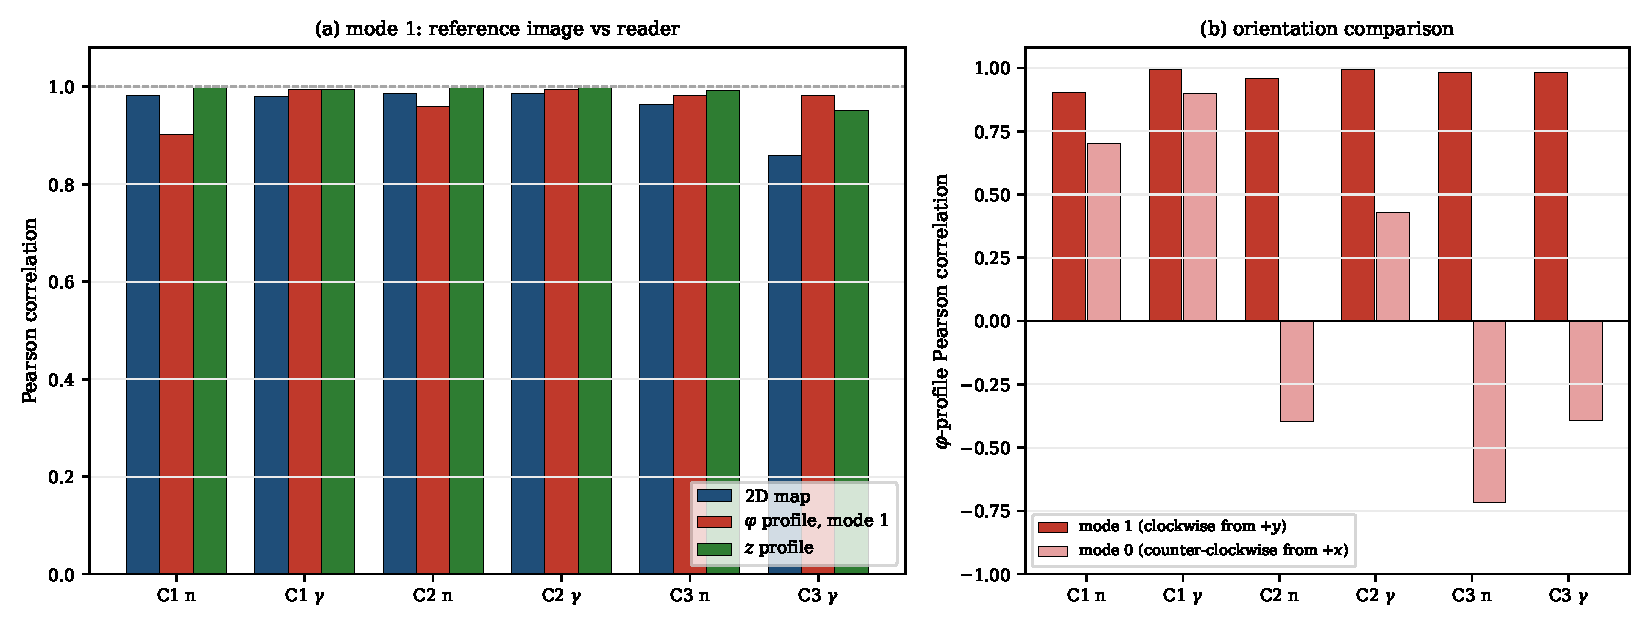
\includegraphics[width=0.95\linewidth]{fig_validation_scores.pdf}
\caption{(a) Correlation between the reference image and the reader map for all
six files: 2D particle/s map, 2D $H^*(10)$ map, $\varphi$ profile in mode~1,
and $z$ profile.
(b) $\varphi$-profile correlation for mode~1 and mode~0.  Mode~1 is higher for
every file; the mode~0 correlation is negative for Cask~2 neutrons, Cask~3
neutrons, and Cask~3 gamma.  Within each file bin the markers are offset
horizontally so that nearly equal scores remain separately visible.}
\label{fig:scores}
\end{figure}

\subsection{Dose-weighted comparison}

The reader writes a second fine map, \texttt{hPhiZ\_dose\_fine}, in which each
record contributes $w\,H^*(10)(E)$ instead of $w$.  The coefficients are the
ICRP~74/ICRU~57 ambient dose equivalent values described in
Section~\ref{sec:part1}; the map is evaluated per record before binning, so the
energy spectrum of each $\varphi$--$z$ cell is weighted separately.  The map is
stored raw; for display it is divided by the source histories $|np|$ and by the
bin area and converted to $\mu$Sv\,h$^{-1}$, with no per-maximum normalisation.
The reference tally area and estimator are not in the WSSA file, so this
per-history display inherits that uncertainty; a surface-crossing weight is not
a dose at a point.  Its absolute scale is reported separately in
Section~\ref{sec:absolute_scale}.  The assumption that the printed \texttt{gDL}/\texttt{nDL}
scales are $H^*(10)$ is stated in Section~\ref{sec:part1}.  The ratio
$h^{H^*(10)}_{\varphi z}/h_{\varphi z}$ has a 12\% RMS variation for Cask~3
gamma and 20\% for the neutrons: the local energy spectrum is similar across
the map, so the per-record coefficient mostly rescales the map rather than
changing its shape.  The reference's smooth baseline is present in neither the
particle/s nor the $H^*(10)$ map.

The particle/s columns in Table~\ref{tab:validation_dose} are therefore not a
dose comparison; they test the geometry and orientation of the source map.  The
$H^*(10)$ columns are the dose-shape comparison, but they are not a one-to-one
validation.  A perfect correlation would require
\(d_b=\alpha r_b+\beta\) in every bin, where \(d_b\) is the reader dose map and
\(r_b\) is the reference map.  A coefficient \(h(E)\) that is constant at all
energies is sufficient but not necessary: a spatially constant energy spectrum
also makes \(d_b\) proportional to the particle map.  What matters is the
bin-averaged coefficient
\(\bar h_b=\sum_i w_i h(E_i)/\sum_i w_i\), not the energy dependence alone.
Peak normalisation removes only a global factor and cannot remove bin-to-bin
variation of \(\bar h_b\).  Even with the correct coefficient, image
digitisation, the unknown reference tally geometry and location, and the
unknown source normalisation prevent a correlation of exactly one.  If the
reference is effective dose rather than \(H^*(10)\), the coefficient itself is
the wrong one, and the comparison is only qualitative.

Table~\ref{tab:validation_dose} compares the particle/s and $H^*(10)$
correlations.  The $H^*(10)$ weighting changes the 2D scores by at most 0.008.
It raises Cask~3 gamma from 0.859 to 0.867; the other five maps remain between
0.989 and 0.999.  The Cask~3 gamma high-pass score is 0.976, essentially the
same as the unweighted 0.978, so the smooth baseline that dominates the raw
score is not removed by the energy weighting.  The $H^*(10)$ maps for all six
files are shown in Figure~\ref{fig:data_all_dose}; the Cask~3 comparison is in
Figure~\ref{fig:maps_dose}.

\begin{table}[H]
\centering
\caption{Pearson correlations for the particle/s map and the $H^*(10)$-weighted
map.  The 2D and profile columns use the reference's native 72$\times$80 grid;
the profile is the mean over the other coordinate.  The $H^*(10)$ columns use
the same grid; the profile correlations are scale-invariant.  The
particle/s columns are a geometry and orientation check; the $H^*(10)$ columns
are a dose-shape comparison under the stated \(H^*(10)\) assumption, not a
coefficient or absolute-dose validation.  Values are rounded to three
decimals.}
\label{tab:validation_dose}
\footnotesize
\begin{tabular}{@{}l r r r r r r@{}}
\toprule
File & 2D p/s & 2D $H^*(10)$ & $\varphi$ p/s & $\varphi$ $H^*(10)$
     & $z$ p/s & $z$ $H^*(10)$ \\
\midrule
\texttt{Cask1\_gamma}    & 0.989 & 0.989 & 0.996 & 0.995 & 0.994 & 0.995 \\
\texttt{Cask1\_neutrons} & 0.998 & 0.999 & 0.981 & 0.980 & 0.999 & 1.000 \\
\texttt{Cask2\_gamma}    & 0.998 & 0.997 & 0.994 & 0.993 & 0.999 & 0.999 \\
\texttt{Cask2\_neutrons} & 0.998 & 0.999 & 0.971 & 0.979 & 0.999 & 1.000 \\
\texttt{Cask3\_gamma}    & 0.859 & 0.867 & 0.981 & 0.982 & 0.952 & 0.953 \\
\texttt{Cask3\_neutrons} & 0.992 & 0.997 & 0.995 & 0.996 & 0.992 & 0.998 \\
\bottomrule
\end{tabular}
\end{table}

\begin{figure}[t]
\centering
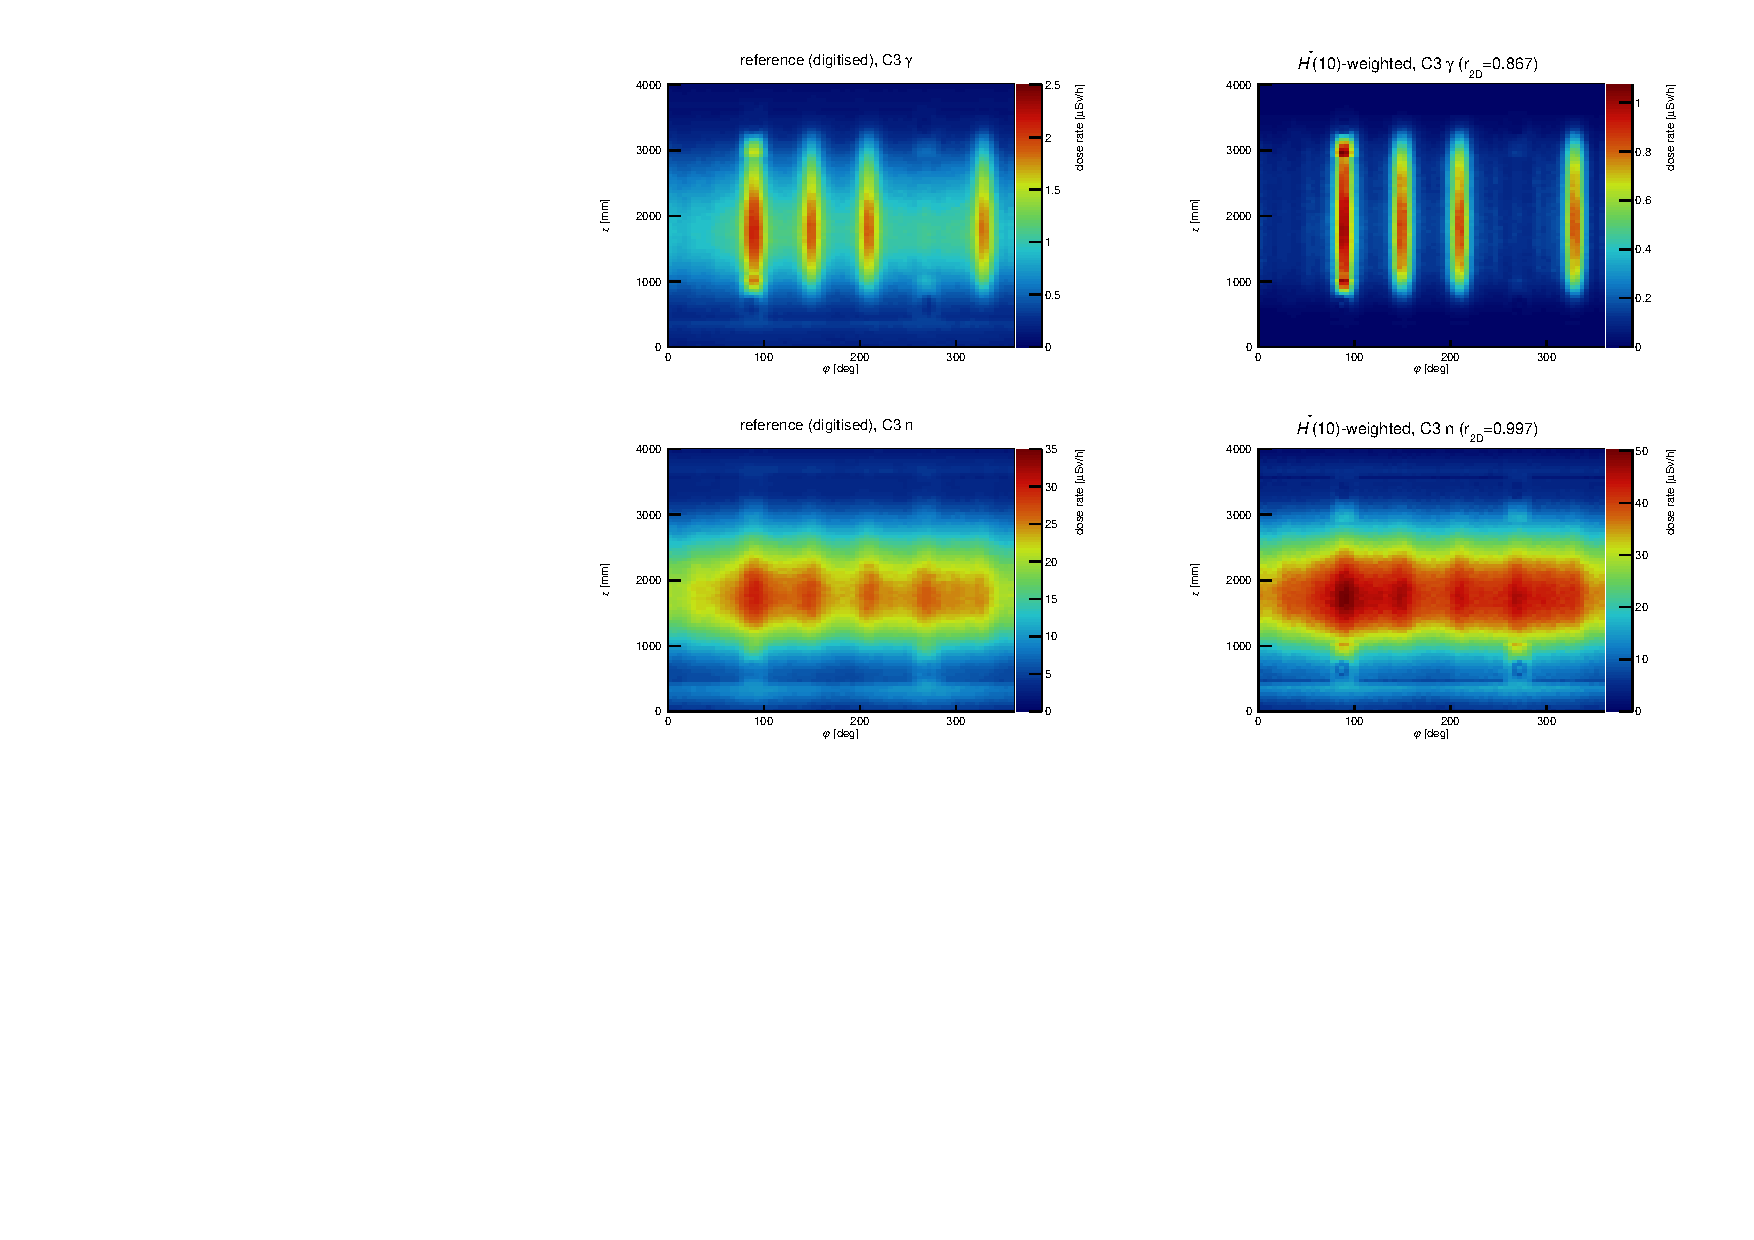
\includegraphics[width=0.92\linewidth]{fig_maps_Cask3_dose.pdf}
\caption{Cask~3 comparison after $H^*(10)$ weighting.  The left column is the
digitised reference and the right column is the $H^*(10)$-weighted reader map;
the top row is gamma and the bottom row is neutrons.  Both columns use
$\mu$Sv\,h$^{-1}$: the left column is the printed reference dose-rate scale,
and the right column is the $H^*(10)$ map divided by $|np|$ and the bin area,
with no per-maximum normalisation.  The reader maxima are within a factor
0.43--1.44 of the reference maxima.  The smooth baseline
between the gamma bands is still present in the reference and still weak in the
reader; the 2D correlations are 0.867 for gamma and 0.997 for neutrons.}
\label{fig:maps_dose}
\end{figure}

\subsection{Energy spectra}

Figure~\ref{fig:energy} shows the weighted energy spectra for all three casks
and both particle types.  The gamma panels use the 200 linear 20~keV bins of
\texttt{hE\_linear} on a linear energy axis; the neutron panels use the 120
log-spaced bins of \texttt{hE} on a logarithmic energy axis.  Both ordinates are
logarithmic sums of MCNP weights per bin.  The gamma spectra extend to
3.65--3.95~MeV; the neutron spectra extend to 19.55--20.44~MeV.  In all six files
the log-bin histogram integral equals the full-file weight sum, and every
record falls inside the range.  The gamma linear histogram is the same record
set restricted to 0--4~MeV; all gamma records lie below 3.95~MeV, so its
integral equals the full weight sum.  The energy plots characterise the files;
no independent energy reference is supplied, so they are not a separate
validation.

\begin{figure}[t]
\centering
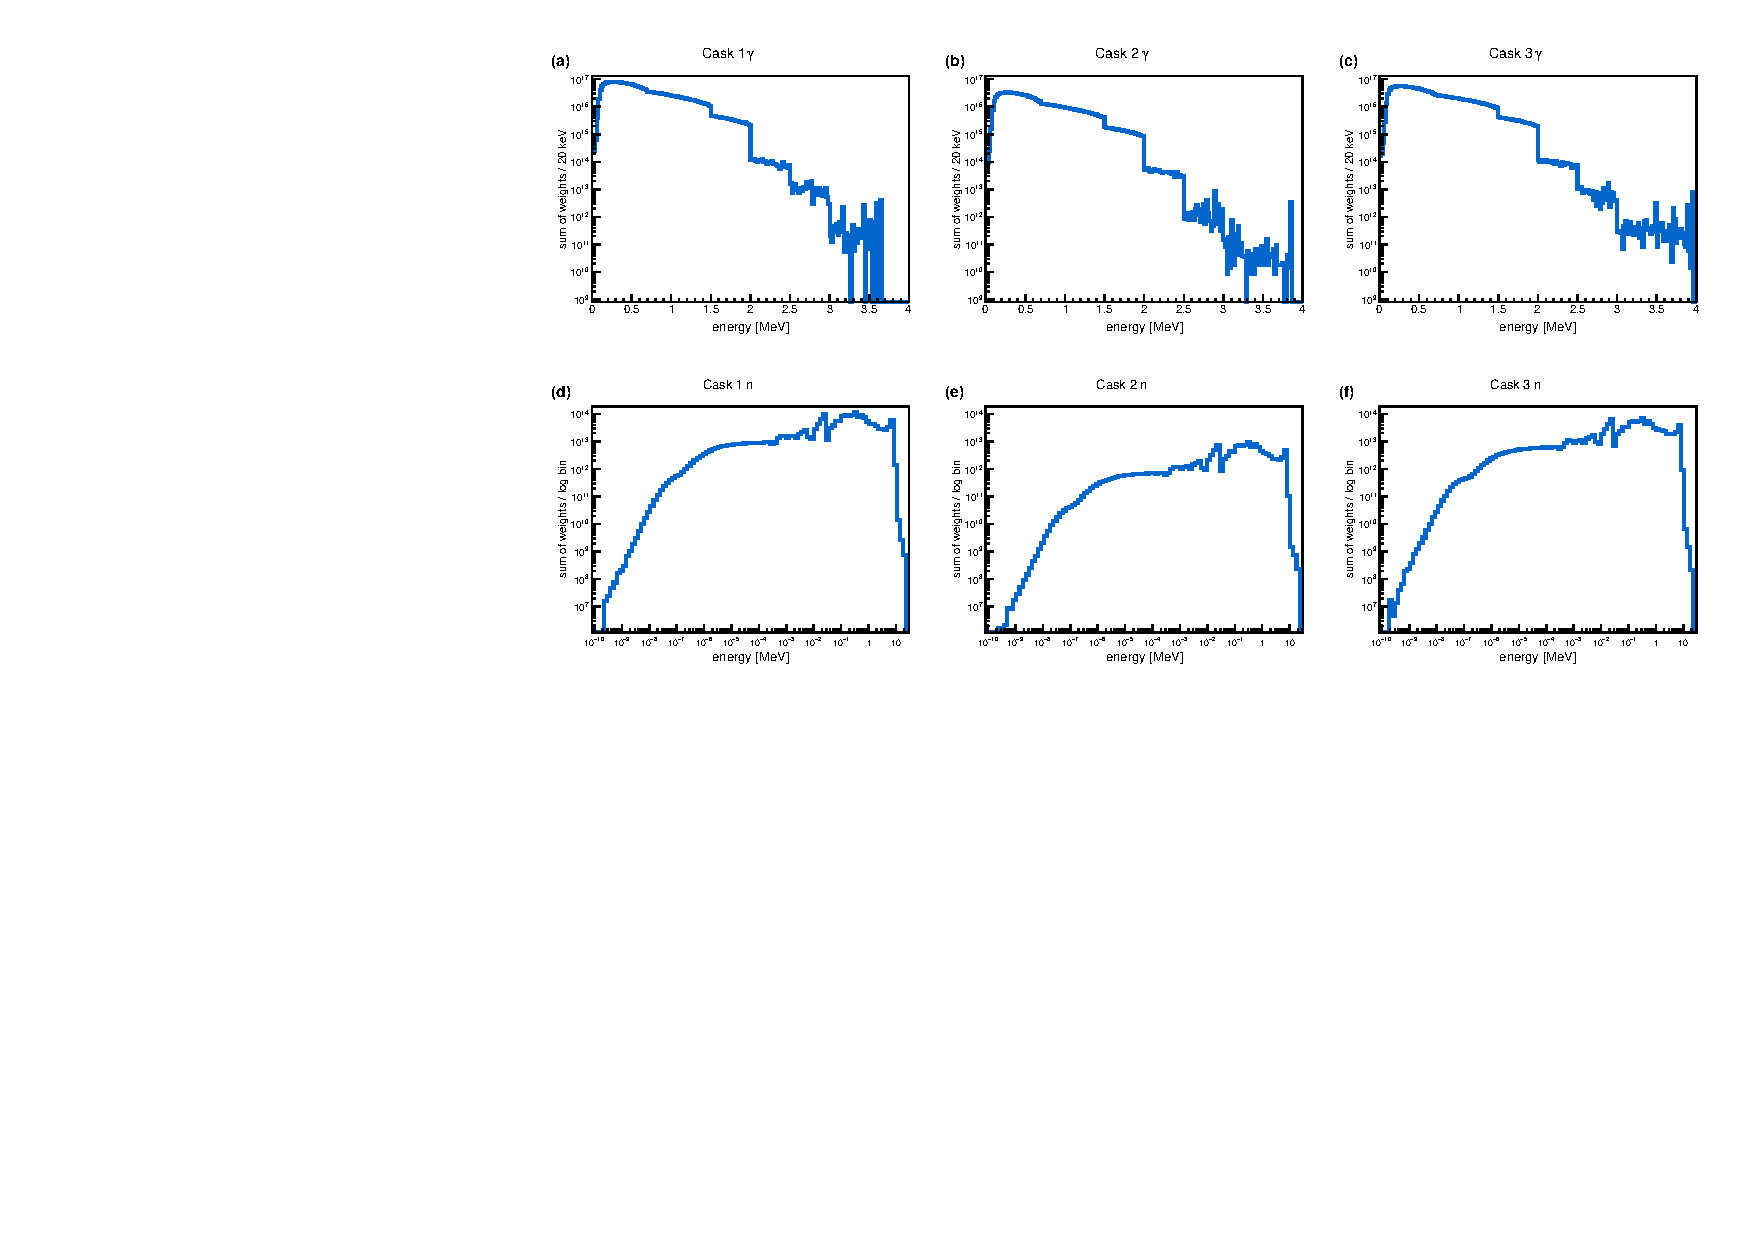
\includegraphics[width=\linewidth]{fig_energy_all.pdf}
\caption{Weighted energy spectra from the full-file passes: (a)--(c) gamma for
Casks~1--3 on a linear energy axis with 20~keV bins; (d)--(f) neutrons for
Casks~1--3 on a logarithmic energy axis with the 120 log-spaced bins.  Both
ordinate scales are logarithmic and show the sum of MCNP weights per bin.  The
gamma and neutron panels use different bin widths; they are not plotted as
counts per unit energy.  The spectra characterise the source files and are not
an independent validation.}
\label{fig:energy}
\end{figure}

Figure~\ref{fig:p1_energy_compare} compares the normalized energy shapes of
WSSA Cask~1 with the Geant4 p1 surface source.  WSSA has no Cask~0 file, so
Cask~1 is the first cask available.  The p1 spectrum is built from the first
$2\times10^{6}$ entries of each of the 70 files and scaled by the source rates
in Table~\ref{tab:p1_wssa}; the WSSA spectrum uses the full file.  Both
histograms are divided by their own integrals, so only the shapes are compared.
The gamma panel uses the 20~keV bins of \texttt{hE\_linear} and the neutron
panel uses the 120 log-spaced bins of \texttt{hE}.  The gamma shapes agree
within a factor of about two below 0.6~MeV; between 0.65 and 1.5~MeV p1 is
lower by a factor 3--4.  WSSA falls steeply after 2~MeV, while p1 keeps a
continuum to 4~MeV.  The neutron shapes agree within about 1.25 up to 1~MeV;
above 2~MeV p1 has a broad shoulder to 18~MeV, while WSSA has a narrow
high-energy spike near 8~MeV.

\begin{figure}[t]
\centering
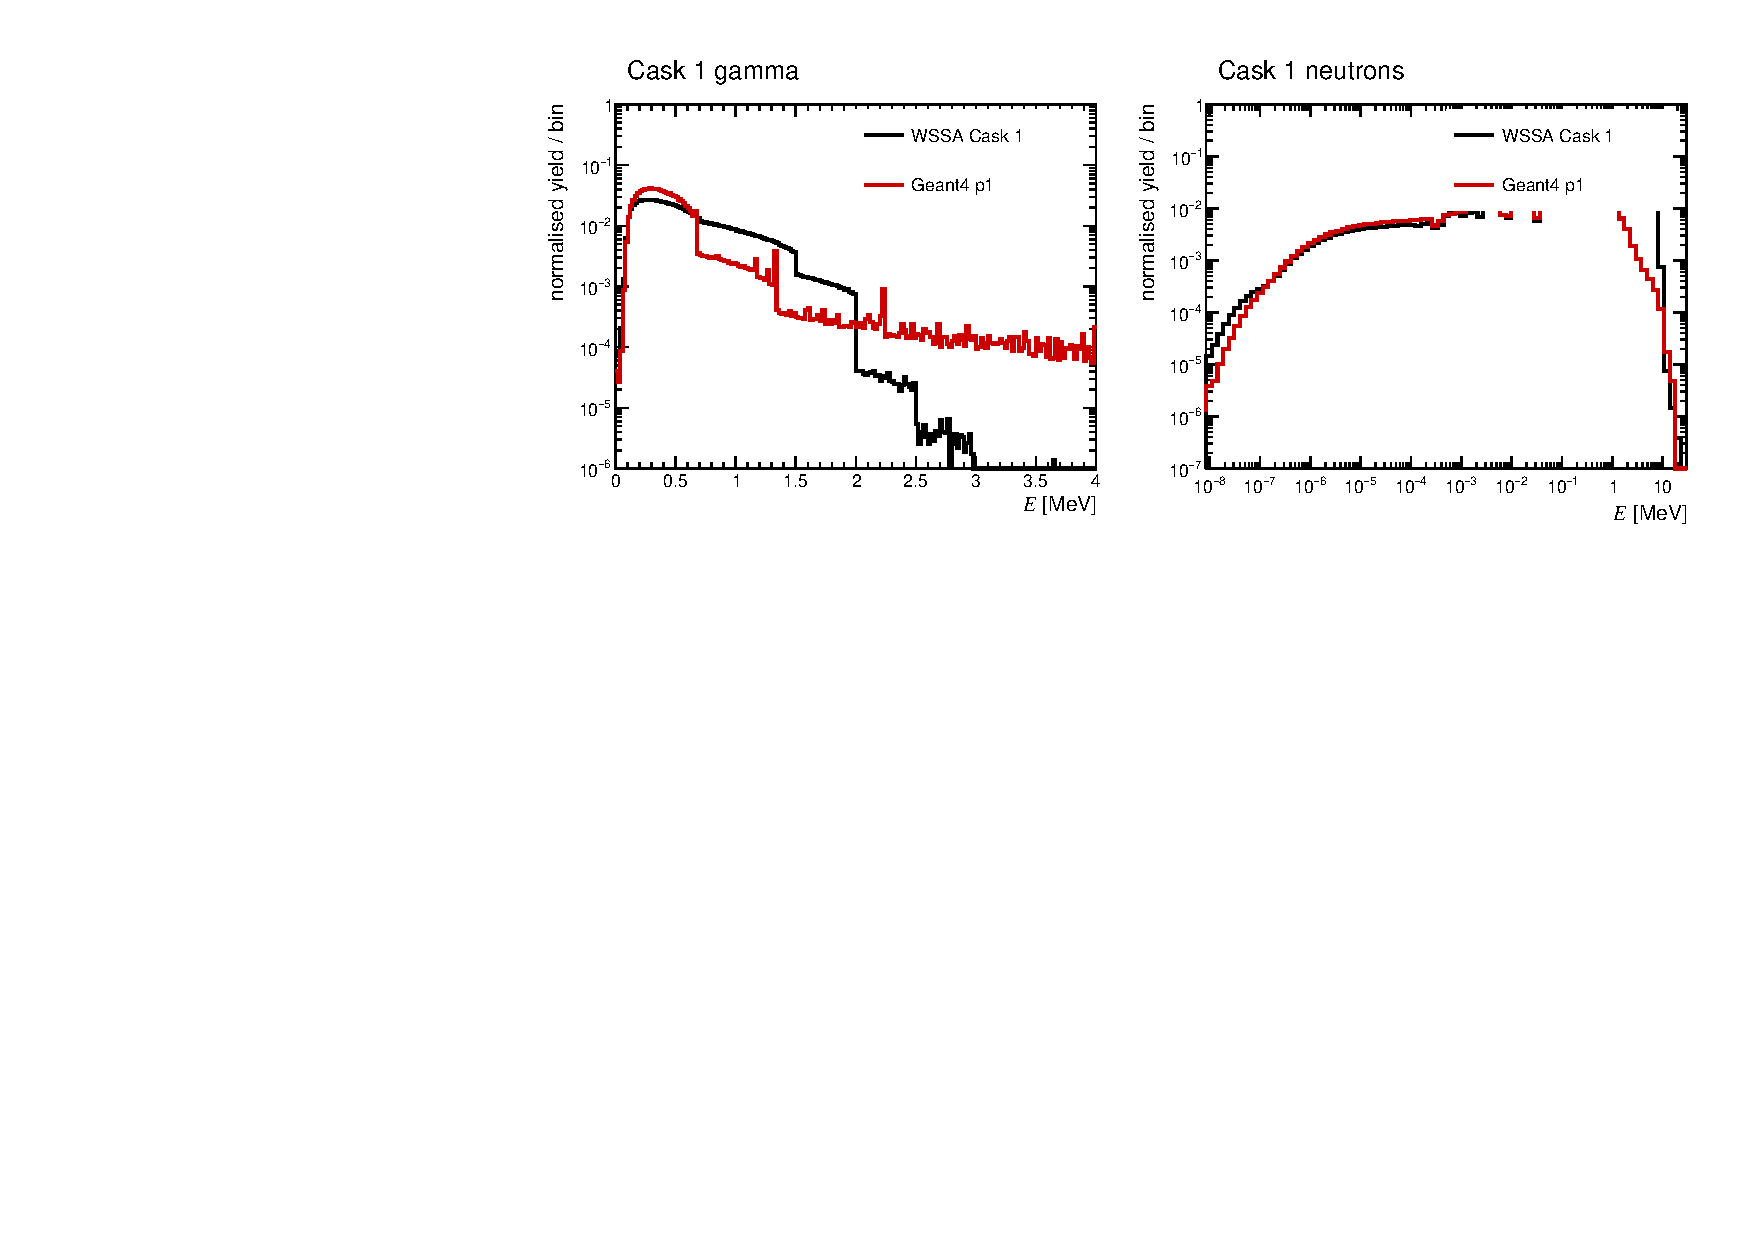
\includegraphics[width=\linewidth]{fig_p1_energy_compare.pdf}
\caption{Normalized energy spectra for WSSA Cask~1 (black) and Geant4 p1
(red).  Gamma is left and neutrons are right.  Each histogram is divided by
its own integral, so the ordinate is a shape density, not a rate.  The gamma
panel uses 20~keV bins on a linear energy axis; the neutron panel uses 120
log-spaced bins on logarithmic axes.  WSSA has no Cask~0 file, so Cask~1 is
the first cask.  The p1 entries are a leading prefix of each of the 70 files;
no independent energy reference is available.}
\label{fig:p1_energy_compare}
\end{figure}

% ---------------------------------------------------------------------------
\section{Part 2: Geant4 replay}\label{sec:part2}

\subsection{Loader and reservoir}

\texttt{SurfaceFluxSampler::LoadWSSA} uses the same \texttt{WSSAReader} in a
single sequential pass.  It reads all \texttt{nrsw} records and keeps a uniform
reservoir sample of at most
\[
  N_{\max} = \min(\texttt{wssaMaxEntries},\,\texttt{nrsw}).
\]
The default \texttt{wssaMaxEntries} is $10^{7}$; a value $\le0$ keeps every
record.  The reservoir uses Algorithm~R: the first $N_{\max}$ valid records are
kept, and each later valid record replaces a uniformly chosen slot with
probability $N_{\max}/n_{\mathrm{valid}}$.  The random generator is seeded with
12345.  The reservoir is uniform over the valid records, so scaling its weight
sum by $n_{\mathrm{valid}}/N_{\mathrm{sample}}$ estimates the full-file weight:
\[
  \texttt{fKeptWeightTotal} =
  \begin{cases}
    \displaystyle \texttt{sumW}\,
      \frac{n_{\mathrm{valid}}}{N_{\mathrm{sample}}}, & N_{\mathrm{sample}}<n_{\mathrm{valid}},\\[6pt]
    \texttt{sumW}, & N_{\mathrm{sample}}=n_{\mathrm{valid}}.
  \end{cases}
\]
The loader prints this estimate, the retained surface counts, and the number of
skipped or marked records.

A record is valid if its reconstructed direction has non-zero magnitude
($\sqrt{u^2+v^2+w^2}>0$).  Degenerate directions are skipped.  A non-positive
weight is clamped to zero but the record is kept and counted separately; the
alias table gives it zero probability.  If every retained weight is zero, the
alias builder falls back to a uniform distribution.  The positions are converted
from cm to mm and shifted by $-H/2$; the direction is normalised.  The surface
classification uses the header:
\begin{itemize}
  \item \texttt{type}=15 $\rightarrow$ side (surface~0);
  \item \texttt{type}=4 and \texttt{coeff}$\ge0$ $\rightarrow$ top (surface~1);
  \item \texttt{type}=4 and \texttt{coeff}$<0$ $\rightarrow$ bottom (surface~2);
  \item any other type, or an identifier absent from the header, $\rightarrow$
        side (surface~0), with an unknown-surface counter.
\end{itemize}
The header in these files has no bottom surface, so the bottom branch is not
exercised by the six files.  The loader sets
\texttt{fKeepRecordedPosition=true}; \texttt{Sample()} therefore keeps the
recorded side and cap positions instead of projecting them onto the Geant4 cap.
This is what preserves the 9~mm top-plane difference described in
Section~\ref{sec:format}.

The alias table is built from the retained weights.  \texttt{Sample()} draws a
uniform slot, compares the fractional part with that slot's alias probability,
and selects either the slot or its alias.  It returns \texttt{weight=1.0}: the
input weight is carried by the alias probabilities, not by the primary weight.
The default $10^{7}$ reservoir is bounded in memory; the retained
\texttt{Crossing} is 40~bytes and the alias arrays add 12~bytes per entry, so
the default sample is roughly half a gigabyte.  The six files have
$1.19\times10^{8}$--$5.64\times10^{8}$ records, so the default cap is a
reservoir, not a full-file cache.

\subsection{Source mode and commands}

The WSSA source mode reuses the existing external-surface vertex path.  The
sampler returns a cask-local position and direction; the primary generator
applies the selected cask rotation and translation, sets the particle from the
PDG code, and writes the primary vertex.  The primary tree therefore stores global coordinates after
the cask rotation, not the raw WSSA coordinates.  The cask index and the optional
$z$ rotation are the same controls used by the CSV and TTree replay modes.

\begin{table}[t]
\centering
\caption{WSSA replay commands.  The file, particle type, and reservoir cap are
the required settings.  The radial and tolerance arguments of the sampler are
not used for WSSA; the loader uses the cask height for the $z$ shift and keeps
the recorded positions.  The normalization command applies only to
\texttt{startRun}.}
\label{tab:commands}
\footnotesize
\begin{tabular}{@{}l l p{7.4cm}@{}}
\toprule
Command & Default & Purpose \\
\midrule
\texttt{/dcs-monitor/surf/wssaFile} & -- & path to the \texttt{.wssa} file; selects WSSA input \\
\texttt{/dcs-monitor/surf/wssaMaxEntries} & 10\,000\,000 & reservoir cap; $\le0$ retains all \\
\texttt{/dcs-monitor/surf/wssaPid} & 0 & 2112 for neutrons, 22 for gammas; 0 infers from the filename \\
\texttt{/dcs-monitor/surf/wssaAbsoluteWeight} & true & true: raw weights are absolute particles/s; false: per-source-history weights \\
\texttt{/dcs-monitor/surf/sourcePid} & 0 & PDG filter; 0 means any \\
\texttt{/dcs-monitor/gun/sourceMode} & -- & set to \texttt{CASTOR440\_surface\_from\_WSSA} \\
\texttt{/dcs-monitor/surf/caskNum} & 0 & cask index used for placement \\
\texttt{/dcs-monitor/surf/sourceRotZ} & 0 & rotate the source about $+z$ (C6 hexant reuse) \\
\texttt{/dcs-monitor/surf/smearPhi}, \texttt{smearZ}, & 0 & optional resampling widths \\
\texttt{smearAngle}, \texttt{smearEfrac} & & \\
\texttt{/dcs-monitor/surf/numPrimaries} & -- & set by the user for the p1 \texttt{startRun} normalisation \\
\texttt{/dcs-monitor/surf/startRun} & -- & compute primaries from the selected WSSA normalization \\
\bottomrule
\end{tabular}
\end{table}

The replay is analog.  The WSSA file already contains the MCNP source weights,
and the alias table carries them; adding importance biasing would apply a second
weighting and is not supported for this mode.  Do not pass \texttt{--biasing}
with \texttt{CASTOR440\_surface\_from\_WSSA}.

\subsection{Smoke tests}

Two 20-event tests verify the full path.  The neutron test uses a 20-event copy
of the CLYC template macro with \texttt{Cask3\_neutrons.wssa} and a
10\,000-record reservoir.  The gamma test uses a cask-only macro with
\texttt{Cask3\_gamma.wssa} and the same cap.  Both write the primary tree and
were checked with a small ROOT macro.

\begin{table}[t]
\centering
\caption{Smoke tests of the WSSA replay.  The load time is the single-threaded
reader time reported by \texttt{TStopwatch} on the local NVMe storage.  The
gamma sample retained 9\,998 side and 2 top records.  The neutron test used the
CLYC detector; the gamma test used only the cask.  The primary tree stores
global coordinates after the cask rotation and translation, so radius and $z$
ranges in the tree are not the raw WSSA ranges.}
\label{tab:tests}
\footnotesize
\begin{tabular}{@{}l r r r r r l r@{}}
\toprule
Test & Records & Retained & Load [s] & Events & PID & Energy [MeV] & $|\vec p|$ \\
\midrule
Neutron & \num{118939773} & \num{10000} & 49.3 & 20 & 2112
        & $2.22\times10^{-6}$--7.73 & 1.000 \\
Gamma   & \num{465772433} & \num{10000} & 214.5 & 20 & 22
        & 0.172--1.859 & 1.000 \\
\bottomrule
\end{tabular}
\end{table}

The neutron test produced 20 primaries with PDG 2112, energies
$2.22\times10^{-6}$--7.73~MeV, and unit direction vectors.  The gamma test
produced 20 primaries with PDG 22, energies 0.172--1.859~MeV, and unit
direction vectors.  The gamma full pass read $4.66\times10^{8}$ records in
214.5~s, about $208~\mathrm{MB\,s^{-1}}$; the retained 10\,000 records are a
small fraction of the file, as intended for a smoke test.  The load time
dominates these 20-event runs; it is not a detector-throughput measurement.

\subsection{Limitations}

The following points bound the conclusions:
\begin{itemize}
  \item The reference maps are dose rate in $\mu$Sv\,h$^{-1}$.  The particle/s
        reader map is a sum of MCNP weights, and the $H^*(10)$ map applies the
        ICRP~74/ICRU~57 coefficient per record.  The sum-of-weights map is
        normalised for the shape comparison; the $H^*(10)$ map is drawn per
        source history in $\mu$Sv\,h$^{-1}$ after the area conversion.  WTI states a source normalisation, but the
        reference tally area and estimator are not in the WSSA file, and a
        surface-crossing weight is not a dose at a point.  The raw absolute map
        is excluded by the diagnostic in Section~\ref{sec:absolute_scale}; the
        per-history map is within a factor 0.43--1.44.
  \item The $H^*(10)$ assignment is an assumption: the supplied images label
        the scales only as \texttt{gDL} and \texttt{nDL}.  If the reference uses
        a different conversion (for example an effective-dose coefficient with a
        stated phantom), the dose-weighted scores will change.  Table~\ref{tab:dose_coeff}
        shows representative differences: \(H^*(10)\) is not effective dose, and
        the AP/ISO effective-dose ratio to \(H^*(10)\) varies with energy.  No
        reference \texttt{DE}/\texttt{DF} card or tally definition was available.
  \item The full pass removes sampling error from the reader maps, but the
        correlations are not an uncertainty budget: the reference is an
        image-derived ordinal map, and neither reader map is an absolute dose
        rate.
  \item The image decoding reduces the colour bar to an ordinal and bins the
        pixels directly to the native 72$\times$80 grid (and the 36$\times$41
        grid for the mode-0 check).  The frame and colour-bar positions are
        detected per image; the scores are not independent of that decoding.
  \item The WSSA top plane is at 4089~mm and the Geant4 cap is at 4080~mm.  The
        loader keeps the recorded positions, so records within 9~mm of the top
        can start above the cap.  The side surface is 2.5~mm outside the fin
        tips.  These are geometric approximations, not format errors.
  \item The reservoir is uniform over valid records; the full-file weight
        estimate assumes that the reservoir is representative.  The alias table
        preserves the relative weights within the retained sample.  The
        \texttt{fKeptWeightTotal} value is an estimate, not an exact sum over
        the file.
  \item The smoke tests use 20 events and a 10\,000-record cap.  They verify the
        loader, particle codes, directions, and energy ranges; they do not
        produce a detector yield or a production statistical uncertainty.
  \item The replay is analog.  Combining it with importance biasing would
        double-weight the source and is not supported.
\end{itemize}

\subsection{Source-rate comparison with the p1 surface flux}

The p1 surface flux and the WSSA full-file sums are both surface crossing
rates, but they are not on the same source normalisation.  The p1 weights were
summed over the 14 base fuels and five sources (70 files), with
\texttt{pid}=22 for gammas and \texttt{pid}=2112 for neutrons, divided by the
file \texttt{nEvts}, and multiplied by the six hexants and the hardcoded
source rates in \texttt{slurm/generate\_p15\_macros.sh}.  The extraction is
reproducible: for the gamma 662 test the p1 sum divided by \texttt{nEvts} is
$1.31\times10^{-8}$, and the p1.5 \texttt{ratio} for the same file is
$1.30\times10^{-8}$.

\begin{table}[t]
\centering
\caption{p1 surface rates and type-resolved WSSA surface multiplicities.  The
p1 rates use the hardcoded source estimates and the six-hexant factor and are
per second.  The WSSA value is the sum of weights divided by $|np|$, separated
by the record type; it is per source history.  The raw sum is the sum of
weights; WTI's stated normalization would imply a crossing rate, but the
per-history column is the one used for the PNG comparison.  The neutron WSSA files contain photons, so the gamma row includes
photons from both the gamma and neutron files.  The two columns have different
units; converting the per-history column to s$^{-1}$ still needs the source
history rate, which is not in the header.}
\label{tab:p1_wssa}
\footnotesize
\begin{tabular}{@{}l l r r@{}}
\toprule
Cask & Particle & $W_{\rm WSSA}$ [per history] & $R_{\rm p1}$ [s$^{-1}$] \\
\midrule
C1 & $\gamma$ & $3.544\times10^{7}$ & $7.504\times10^{7}$ \\
C1 & $n$      & $1.329\times10^{7}$ & $1.609\times10^{7}$ \\
C2 & $\gamma$ & $1.216\times10^{7}$ & $7.504\times10^{7}$ \\
C2 & $n$      & $1.061\times10^{6}$ & $1.609\times10^{7}$ \\
C3 & $\gamma$ & $8.020\times10^{6}$ & $7.504\times10^{7}$ \\
C3 & $n$      & $8.111\times10^{6}$ & $1.609\times10^{7}$ \\
\bottomrule
\end{tabular}
\end{table}

The p1 gamma rate is $7.50\times10^{7}$~s$^{-1}$ and the neutron rate is
$1.61\times10^{7}$~s$^{-1}$.  The 662~keV line supplies
$5.71\times10^{7}$~s$^{-1}$ of the gamma rate; the Watt source supplies the
whole $1.61\times10^{7}$~s$^{-1}$ neutron rate, with only $6\times10^{2}$ and
$1.2\times10^{3}$~s$^{-1}$ from the 1173 and 1332~keV sources.

The WSSA values are per source history; the p1 values are per second.  Applying
WTI's stated normalization literally would make the raw WSSA sums
$1.5\times10^{14}$--$3.0\times10^{18}$~s$^{-1}$ for these files, which is not on
the same scale as the p1 rate ($1.6\times10^{7}$--$7.5\times10^{7}$~s$^{-1}$).
The raw sum is therefore not treated as a validated absolute rate.  The
per-history column is retained because it is within a factor 0.43--1.44 of the
PNG scale; converting it to s$^{-1}$ needs the source history rate, which is not
in the header.  Multiplying the per-history column by that rate gives the
per-second surface rate; the p1/WSSA per-second ratio is then
$R_{\rm p1}/(S W_{\rm WSSA})$.  The p1 surface-flux route can reproduce the p1
spectra and spatial distribution, but matching the WSSA amplitude also needs the
history rate.  The WSSA replay
samples the WSSA spectra and spatial distribution directly and is the more
faithful source; it needs the selected WSSA normalisation, the header $|np|$
divisor for the per-history mode, and the mixed particle-type handling
described in Section~\ref{sec:part2}.

\begin{table}[t]
\centering
\caption{Surface rate and mean energy of the particles leaving the cask.  The
p1 row uses the 84-assembly source and its rate is per second; the WSSA rows
use the type-resolved full-file sums and their rates are per source history.
The p1 mean energies are from representative fuel-0 and fuel-7 surface-flux
files, sampling $2\times10^{7}$ crossings per source; the WSSA means use every
record.  The WSSA gamma values include the photons stored in the neutron
files.  $^{a}$p1 rate in s$^{-1}$; WSSA rate per source history.  Multiply
the WSSA per-history rates by the source history rate for s$^{-1}$.}
\label{tab:mean_energy}
\footnotesize
\begin{tabular}{@{}l r r r r@{}}
\toprule
Model & $\gamma$ rate$^{a}$ & $\langle E_\gamma\rangle$ [MeV]
      & $n$ rate$^{a}$ & $\langle E_n\rangle$ [MeV] \\
\midrule
p1 (84 assemblies) & $7.504\times10^{7}$ & $0.504$ & $1.609\times10^{7}$ & $0.19$--$0.23$ \\
C1 & $3.544\times10^{7}$ & $0.861$ & $1.329\times10^{7}$ & $0.167$ \\
C2 & $1.216\times10^{7}$ & $0.657$ & $1.061\times10^{6}$ & $0.184$ \\
C3 & $8.020\times10^{6}$ & $1.342$ & $8.111\times10^{6}$ & $0.144$ \\
\bottomrule
\end{tabular}
\end{table}

For a 180~s source interval the p1 cask emits $1.35\times10^{10}$ gammas and
$2.90\times10^{9}$ neutrons.  The WSSA values at one source history per second
are $6.38\times10^{9}$ and $2.39\times10^{9}$ for C1, $2.19\times10^{9}$ and
$1.91\times10^{8}$ for C2, and $1.44\times10^{9}$ and $1.46\times10^{9}$ for
C3; multiply these by the source history rate $S$ for the actual
per-second count.  The p1 p2 replay reaches its totals as a sum over its source
and fuel configurations; the WSSA replay uses one cask configuration, split
into chunks if the computed run exceeds the \texttt{/run/beamOn} limit.

The p1 gamma mean is $0.504$~MeV, dominated by the 662~keV source after
Compton scattering: the per-source means are $0.363$~MeV (662~keV),
$0.574$~MeV (1173~keV), $0.643$~MeV (1332~keV), $0.617$~MeV (Eu154), and
$1.652$~MeV for the photons produced by the Watt neutron source.  The WSSA
gamma files alone have means of $0.617$, $0.601$, and $0.640$~MeV; the
$2.16$--$2.17$~MeV photons in the neutron files raise the combined C1 and C3
means to $0.861$ and $1.342$~MeV.  The p1 neutron mean is $0.19$--$0.23$~MeV
from the two sampled bases; the WSSA neutron means are $0.144$--$0.184$~MeV.
The p1 neutron spectrum is therefore slightly harder, while the p1 gamma
spectrum is softer than the WSSA gamma spectrum when the neutron-file photons
are included.

\subsection{p1 aggregate $\varphi$--$z$ maps}\label{sec:p1_maps}

The 70 p1 surface-flux files can also be summed into one cask map.  The
aggregation applies the six C6 hexants to each of the 14 base fuels, rotates
the base map by $60^\circ$ per hexant, and splits the records by
\texttt{pid}=22 for gammas and \texttt{pid}=2112 for neutrons.  Each record is
weighted by its source rate and by the ICRP~74/ICRU~57 $H^*(10)$ coefficient;
the $\varphi$--$z$ bins are the reference $72\times80$ grid.  The p1 body
coordinate is shifted by $+2040$~mm so that the map runs from the bottom to
$4000$~mm.  Each side bin is divided by $55.63$~cm$^2$, and each bottom or
top cap bin by $709.3$~cm$^2$ ($\pi R^2/72$ with $R=127.5$~cm).

The full 70-file set contains $8.2\times10^9$ entries and 529~GB.  The map
shown here reads the first $2\times10^6$ entries of each file and scales each
file's shape to the sum of weights in
\texttt{g4\_p1\_surface\_rates.csv}; this uses $1.4\times10^8$ entries.  The
resulting map rate is $7.482\times10^7$~s$^{-1}$ for gammas and
$1.608\times10^7$~s$^{-1}$ for neutrons, compared with the CSV totals
$7.504\times10^7$ and $1.609\times10^7$~s$^{-1}$ (ratios 0.997 and 0.999).
The small deficit is the top cap at $z=4080$~mm, which lies outside the
reference $0$--$4000$~mm window.

\begin{figure}[t]
\centering
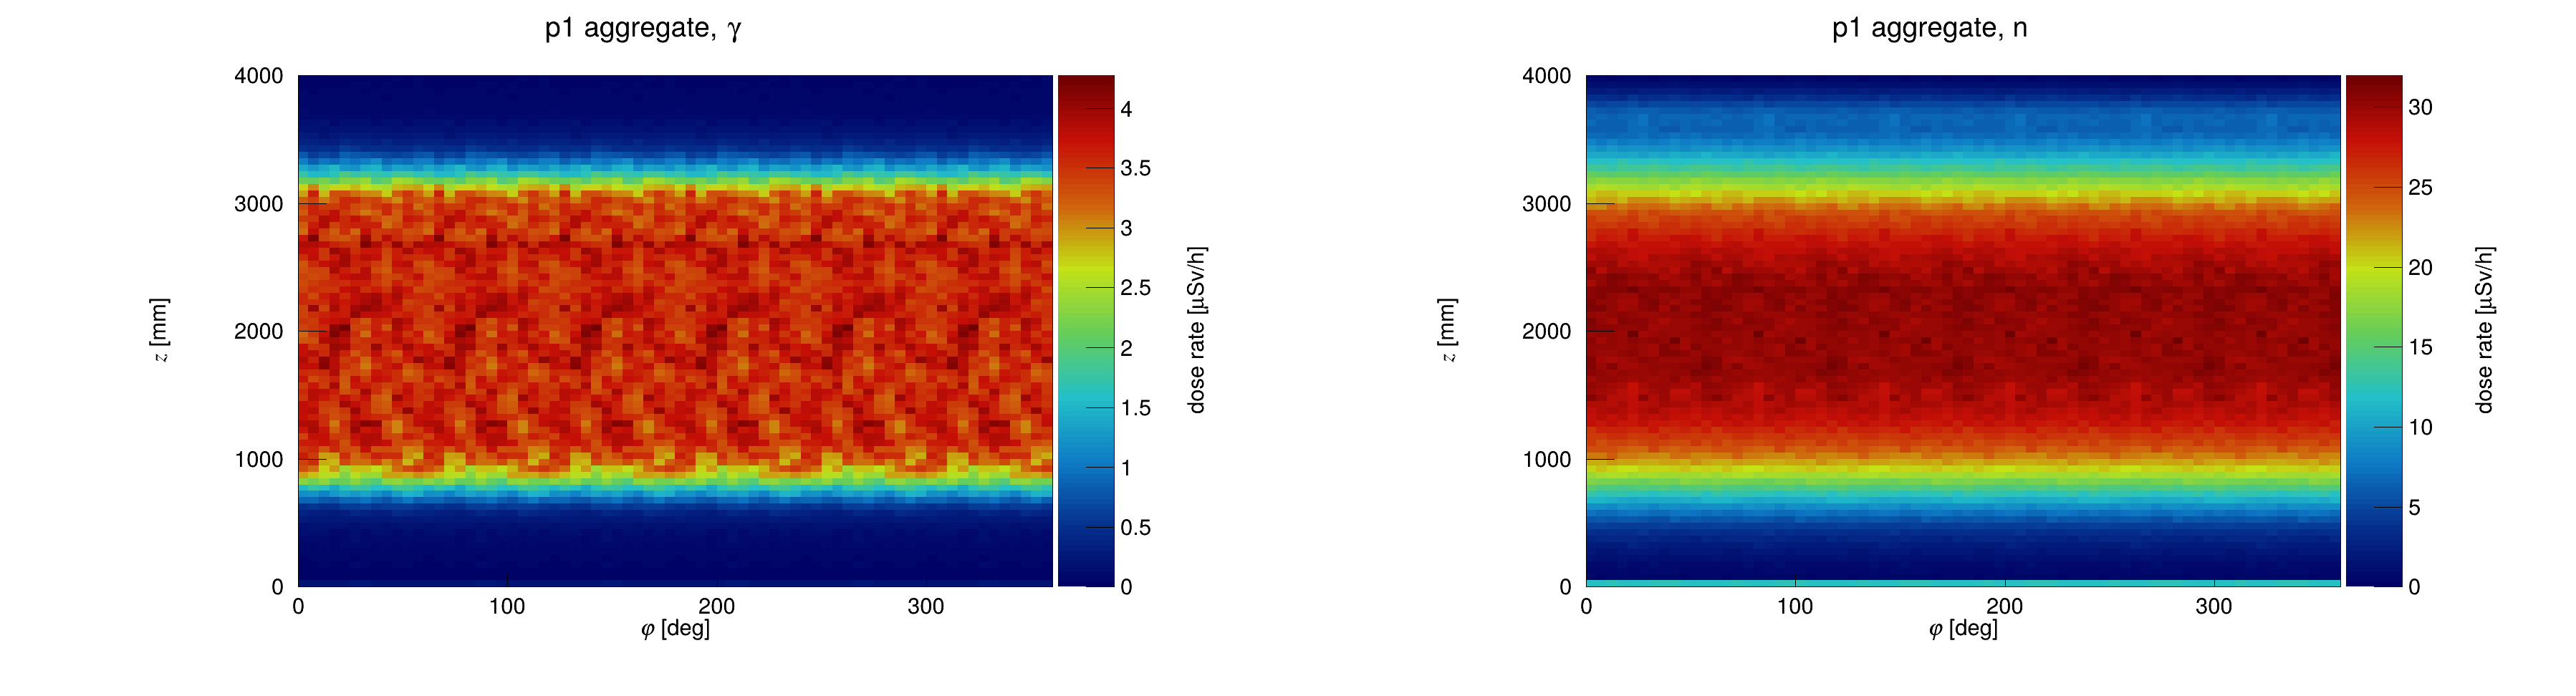
\includegraphics[width=\linewidth]{fig_p1_phi_z_maps.png}
\caption{p1 aggregate $\varphi$--$z$ dose-rate maps after summing all 84 fuel
assemblies: (left) gammas and (right) neutrons.  Both panels use the reference
$72\times80$ grid and the reference $\varphi$ and $z$ ranges.  Each panel has
its own linear $H^*(10)$ colour scale because the maxima differ by a factor
7.5: the gamma maximum is $4.27$~$\mu$Sv\,h$^{-1}$ at
$(\varphi,z)=(22.5^\circ,2025~\text{mm})$, and the neutron maximum is
$32.0$~$\mu$Sv\,h$^{-1}$ at $(22.5^\circ,1975~\text{mm})$.  The isolated row at
$z\approx0$ is the bottom cap projected into one height bin; it is not a
physical azimuthal feature.  The map is a shape cross-check, not a
reproduction of the reference absolute normalisation.}
\label{fig:p1_maps}
\end{figure}

The p1 gamma map is a broad band over $z\approx800$--$3200$~mm, with its
brightest bin at $2025$~mm; the neutron map is a smoother band over
$z\approx700$--$3200$~mm, peaking near $1975$~mm.  Both maps are nearly
uniform in $\varphi$: summing all 84 assemblies fills the ring, so the p1
aggregate does not reproduce the per-cask gamma lobes.  The remaining
bin-to-bin texture in the gamma panel is the $2\times10^6$-entry sampling.
There is no seam at $0^\circ/360^\circ$.  The gamma maximum lies between the
reference Cask~2 and Cask~1 values ($1.4$ and $5$~$\mu$Sv\,h$^{-1}$), while the
neutron maximum is just below the Cask~3 value ($35$~$\mu$Sv\,h$^{-1}$) and
well below Cask~1 ($60$~$\mu$Sv\,h$^{-1}$).  The comparison is therefore useful
for the $z$ extent and the absolute scale, not for the azimuthal lobes: the p1
source is the 84-assembly p1 model, and the reference files are separate cask
configurations with their own source normalisation.

\section{Summary and next steps}

The binary format is understood and implemented once.  The dose convention is
kept as the operational ambient dose equivalent \(H^*(10)\); ``ambient dose''
is a shorthand for this quantity, not a separate conversion table.  Effective
dose would be a different protection quantity and would need a stated phantom
and irradiation geometry.  The offline reader reproduces the supplied
$\varphi$--$z$ structure: the particle/s 2D correlations
are 0.859--0.998, the mode~1 $\varphi$ profiles are 0.971--0.996, and the $z$
profiles are 0.952--0.999.  Applying the ICRP~74/ICRU~57 $H^*(10)$ coefficients
per record gives 2D correlations of 0.867--0.999, $\varphi$ profiles of
0.979--0.996, and $z$ profiles of 0.953--1.000.  Mode~1 (clockwise from $+y$)
is the reference convention for all six files.  The Cask~1 gamma double lobe is
reproduced in the same $5^\circ$ bins.

The lower 2D score of Cask~3 gamma is a smooth-baseline contrast difference, not
a peak shift: the peaks agree within one bin, no one-bin shift improves the
unweighted score by more than 0.004, and a high-pass test raises the unweighted
2D score to 0.978.  The marginal profiles stay high because they average over
the other coordinate.  The $H^*(10)$ weighting raises the raw score only to
0.867 and leaves the high-pass score at 0.976; the smooth baseline is still
missing.  The residual is therefore not explained by the energy dependence of
the flux-to-dose coefficient alone.  It is consistent with a difference in the
reference tally definition or normalisation, or with a contribution that is not
in the surface-crossing record set; separating these needs the reference tally
and its \texttt{DE}/\texttt{DF} cards, which are not in the WSSA file.

The Geant4 path reads the same records, retains a uniform reservoir, builds an
alias table, and returns unit-weight primaries at the recorded positions.  The
neutron and gamma smoke tests confirm the particle codes, unit directions, and
energy ranges.  The gamma full pass demonstrates that the 44.7~GB file can be
read in a few minutes with the default 10M cap.

The next step is a detector-response run with
\texttt{CASTOR440\_surface\_from\_WSSA} for the cask and particle type of
interest, followed by a comparison of the detector tally with the reference
dose map.  The reader now provides both the weight-sum map and the
$H^*(10)$-weighted shape map; the weight-sum map remains the one used for the
Geant4 replay because it preserves the MCNP weights without a second physical
normalisation.  The raw sum follows WTI's stated convention and is the default
replay mode; its absolute scale is not validated here.  The per-history map
needs the source history rate in addition to $|np|$.  An absolute
$\mu$Sv\,h$^{-1}$ comparison also needs the reference tally area and coefficient
card.

% ---------------------------------------------------------------------------
\appendix
\section{Full maps and original references}\label{app:maps}

Figures~\ref{fig:reference_all}, \ref{fig:data_all}, and
\ref{fig:data_all_dose} show the digitised reference maps, the full particle/s
reader maps, and the $H^*(10)$-weighted reader maps for all six files on the
reference's native 72$\times$80 grid; the correlations use the 72$\times$80
grid for the 2D and mode-1 scores and the 36$\times$41 grid for the mode-0
score.
Figure~\ref{fig:orig} reproduces the six supplied PNGs unchanged; the ROOT macro
copies them to \texttt{figures/orig\_*.png}.  The original images contain their
own axes and colour bars; the reference panels use the dose-rate scale of those
bars, the particle/s reader panels are normalised sums of weights, and the
$H^*(10)$ reader panels are per-history dose rates in $\mu$Sv\,h$^{-1}$.

\begin{figure}[p]
\centering
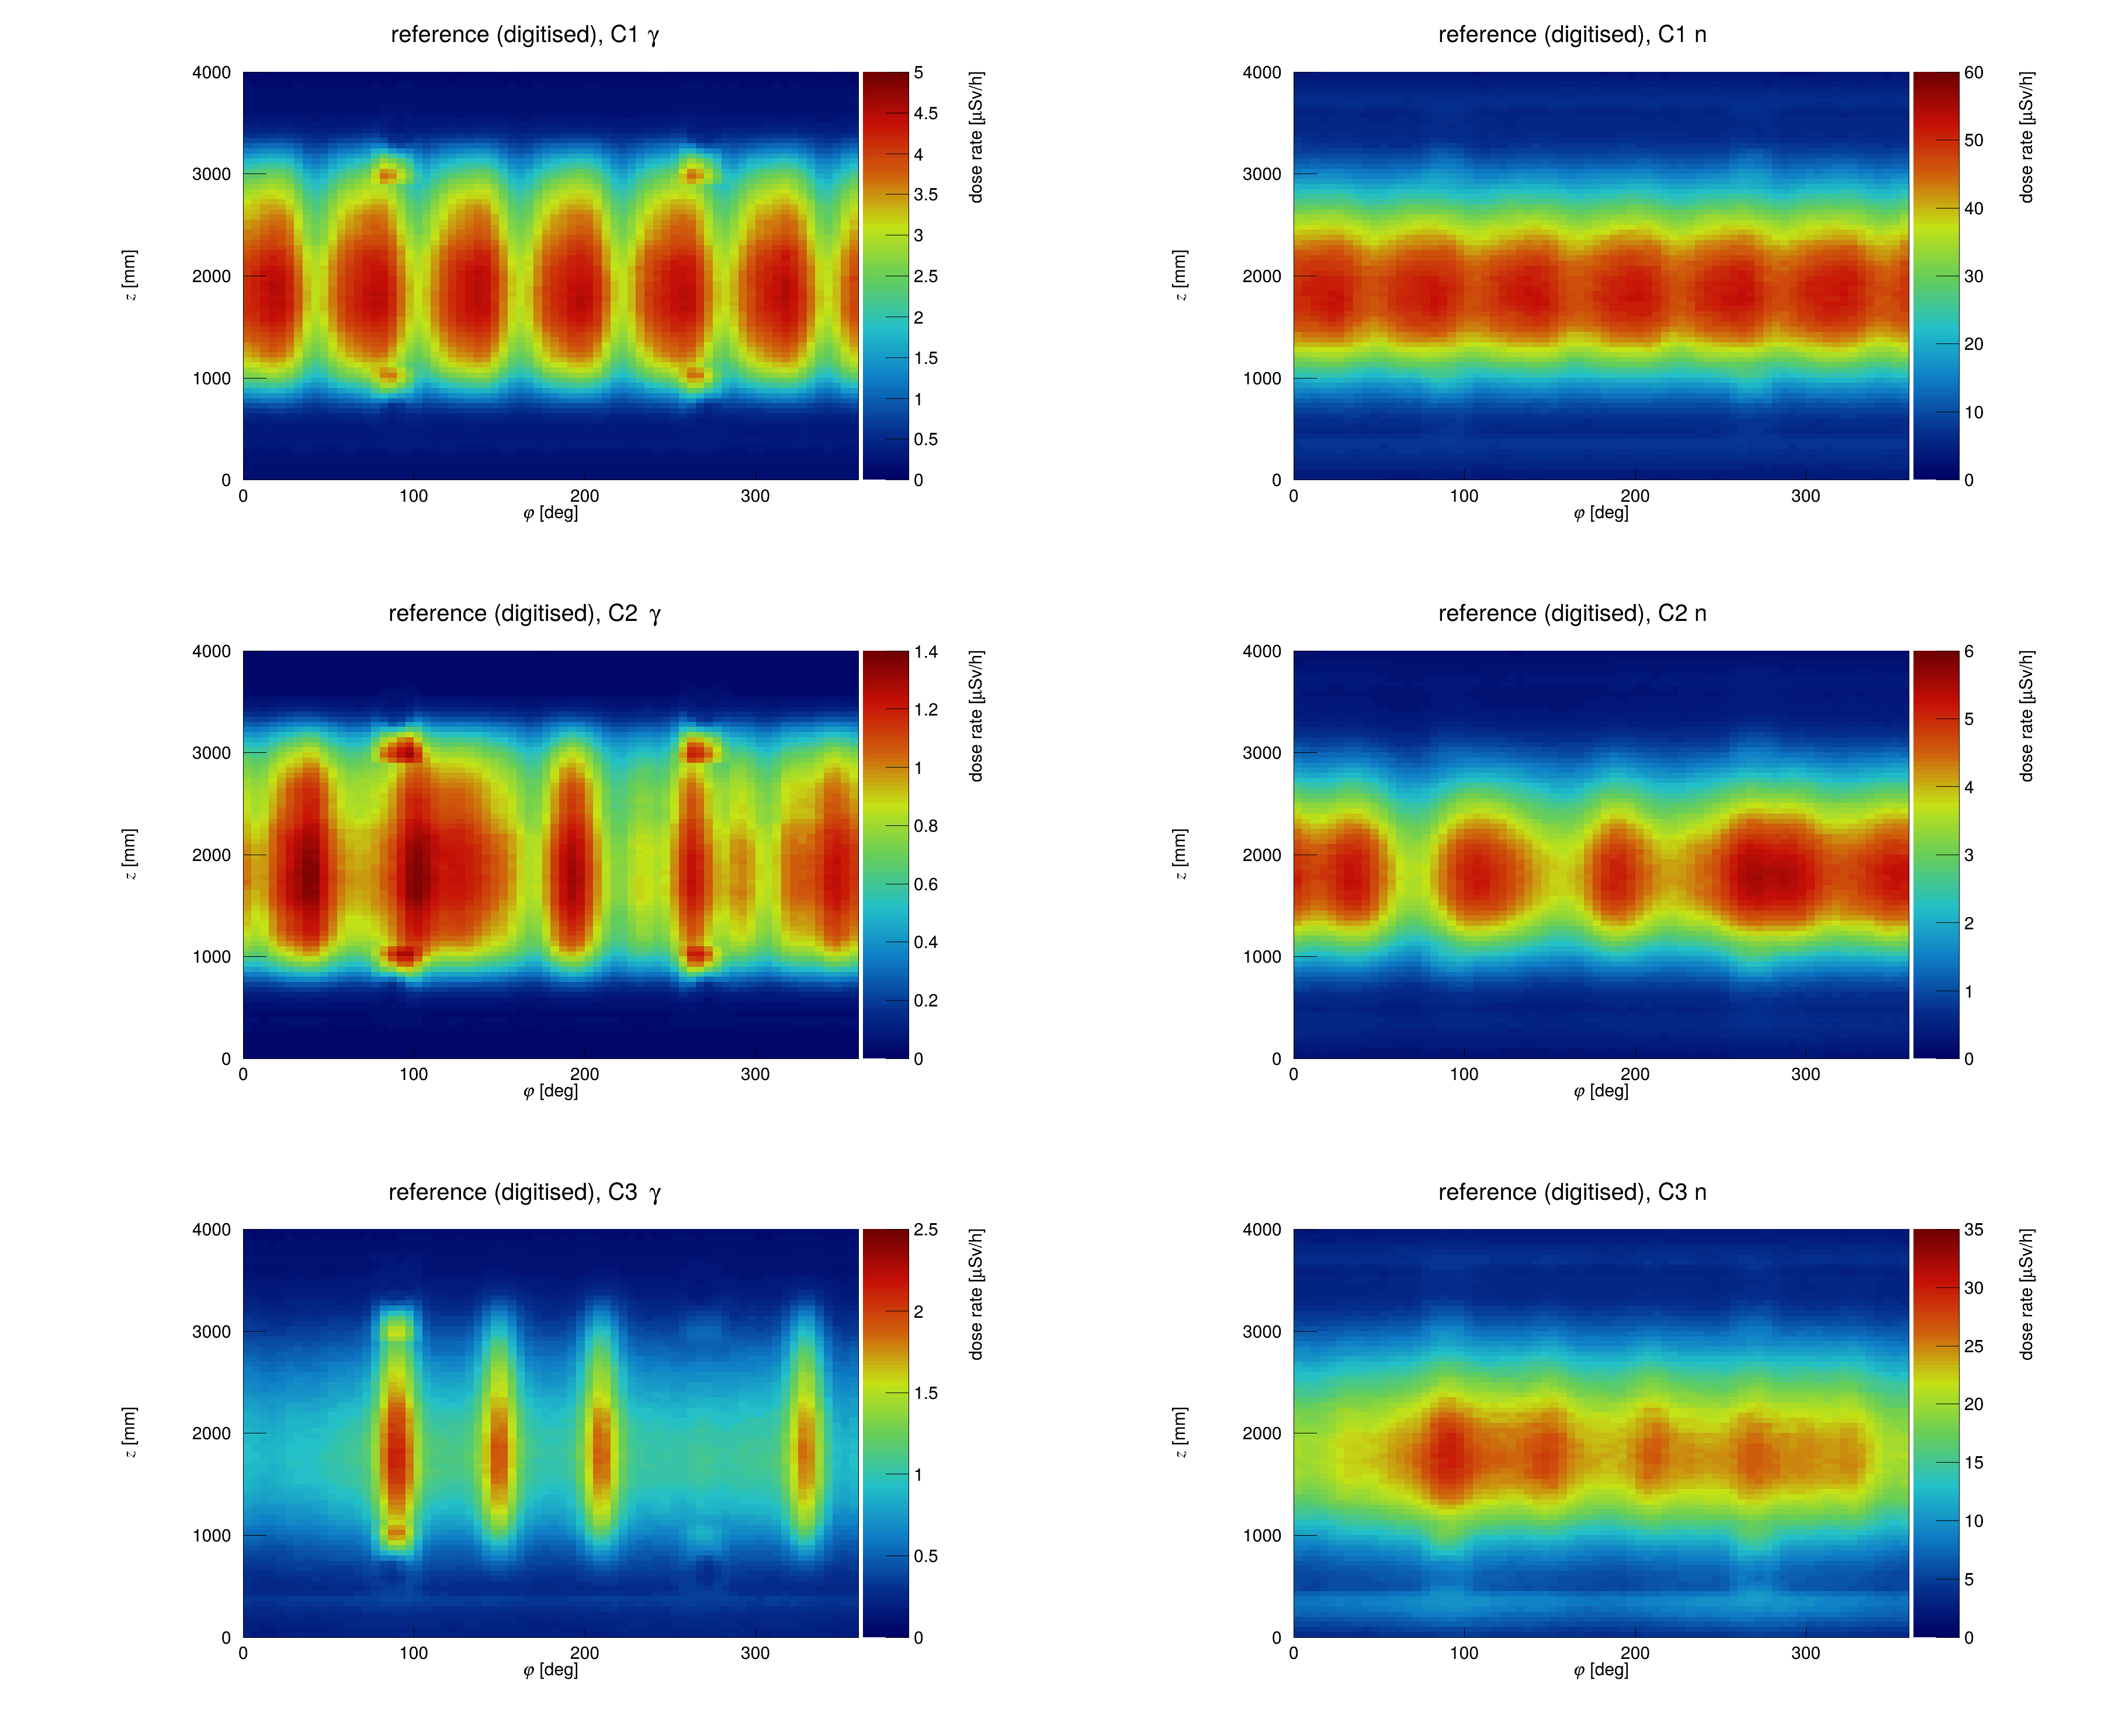
\includegraphics[width=\linewidth]{fig_reference_maps_all.png}
\caption{Digitised reference maps for all six files, drawn on the dose-rate
scale printed on each image's own colour bar ($\mu$Sv\,h$^{-1}$); the colour
bars therefore have different ranges.  Rows are Cask~1, 2, and 3 from top to
bottom; columns are gamma (left) and neutrons (right).  The frame and colour
bar are detected per image; the maps are digitised directly on the native
72$\times$80 grid and on the 36$\times$41 grid for the mode-0 check.  The
originals are in Figure~\ref{fig:orig}.}
\label{fig:reference_all}
\end{figure}

\begin{figure}[p]
\centering
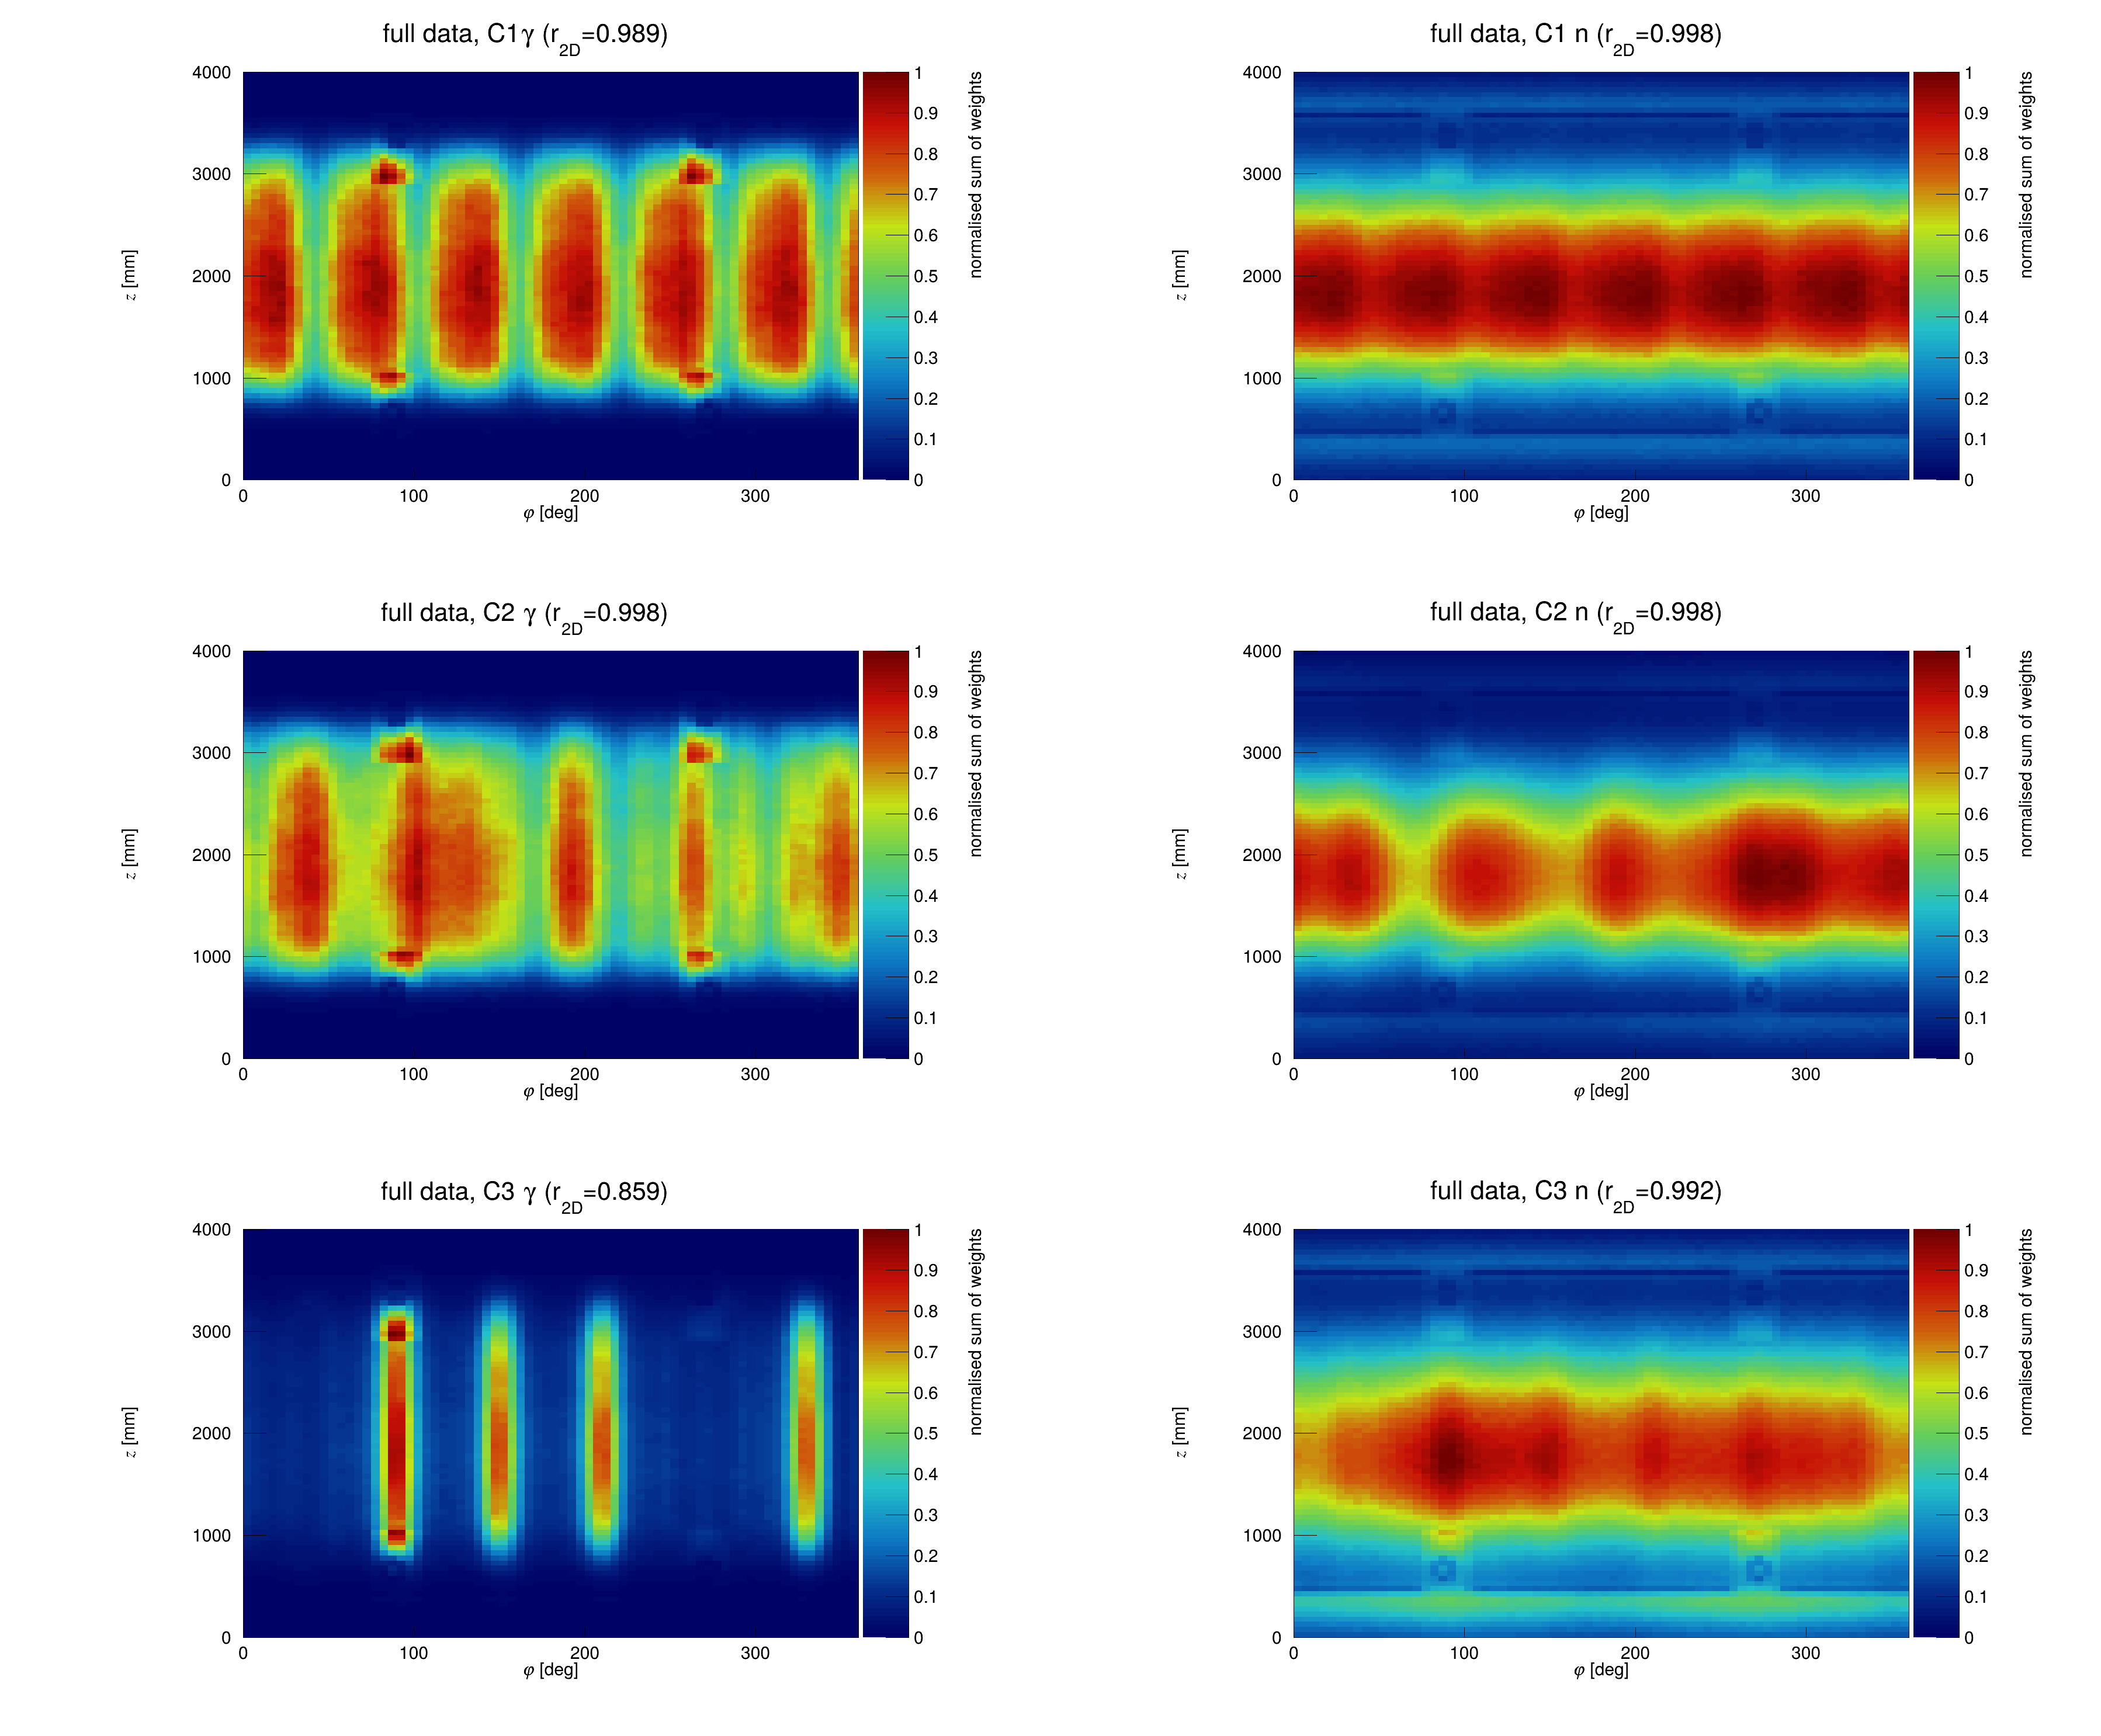
\includegraphics[width=\linewidth]{fig_data_maps_all.png}
\caption{Full-file reader maps for the six WSSA files.  Rows are Cask~1, 2,
and 3 from top to bottom; columns are gamma (left) and neutrons (right).  Each
panel is the sum of MCNP weights normalised to its own maximum on the native
72$\times$80 grid; the title gives the 72$\times$80 correlation with the
digitised reference.  The maps use mode~1 (clockwise from $+y$).}
\label{fig:data_all}
\end{figure}

\begin{figure}[p]
\centering
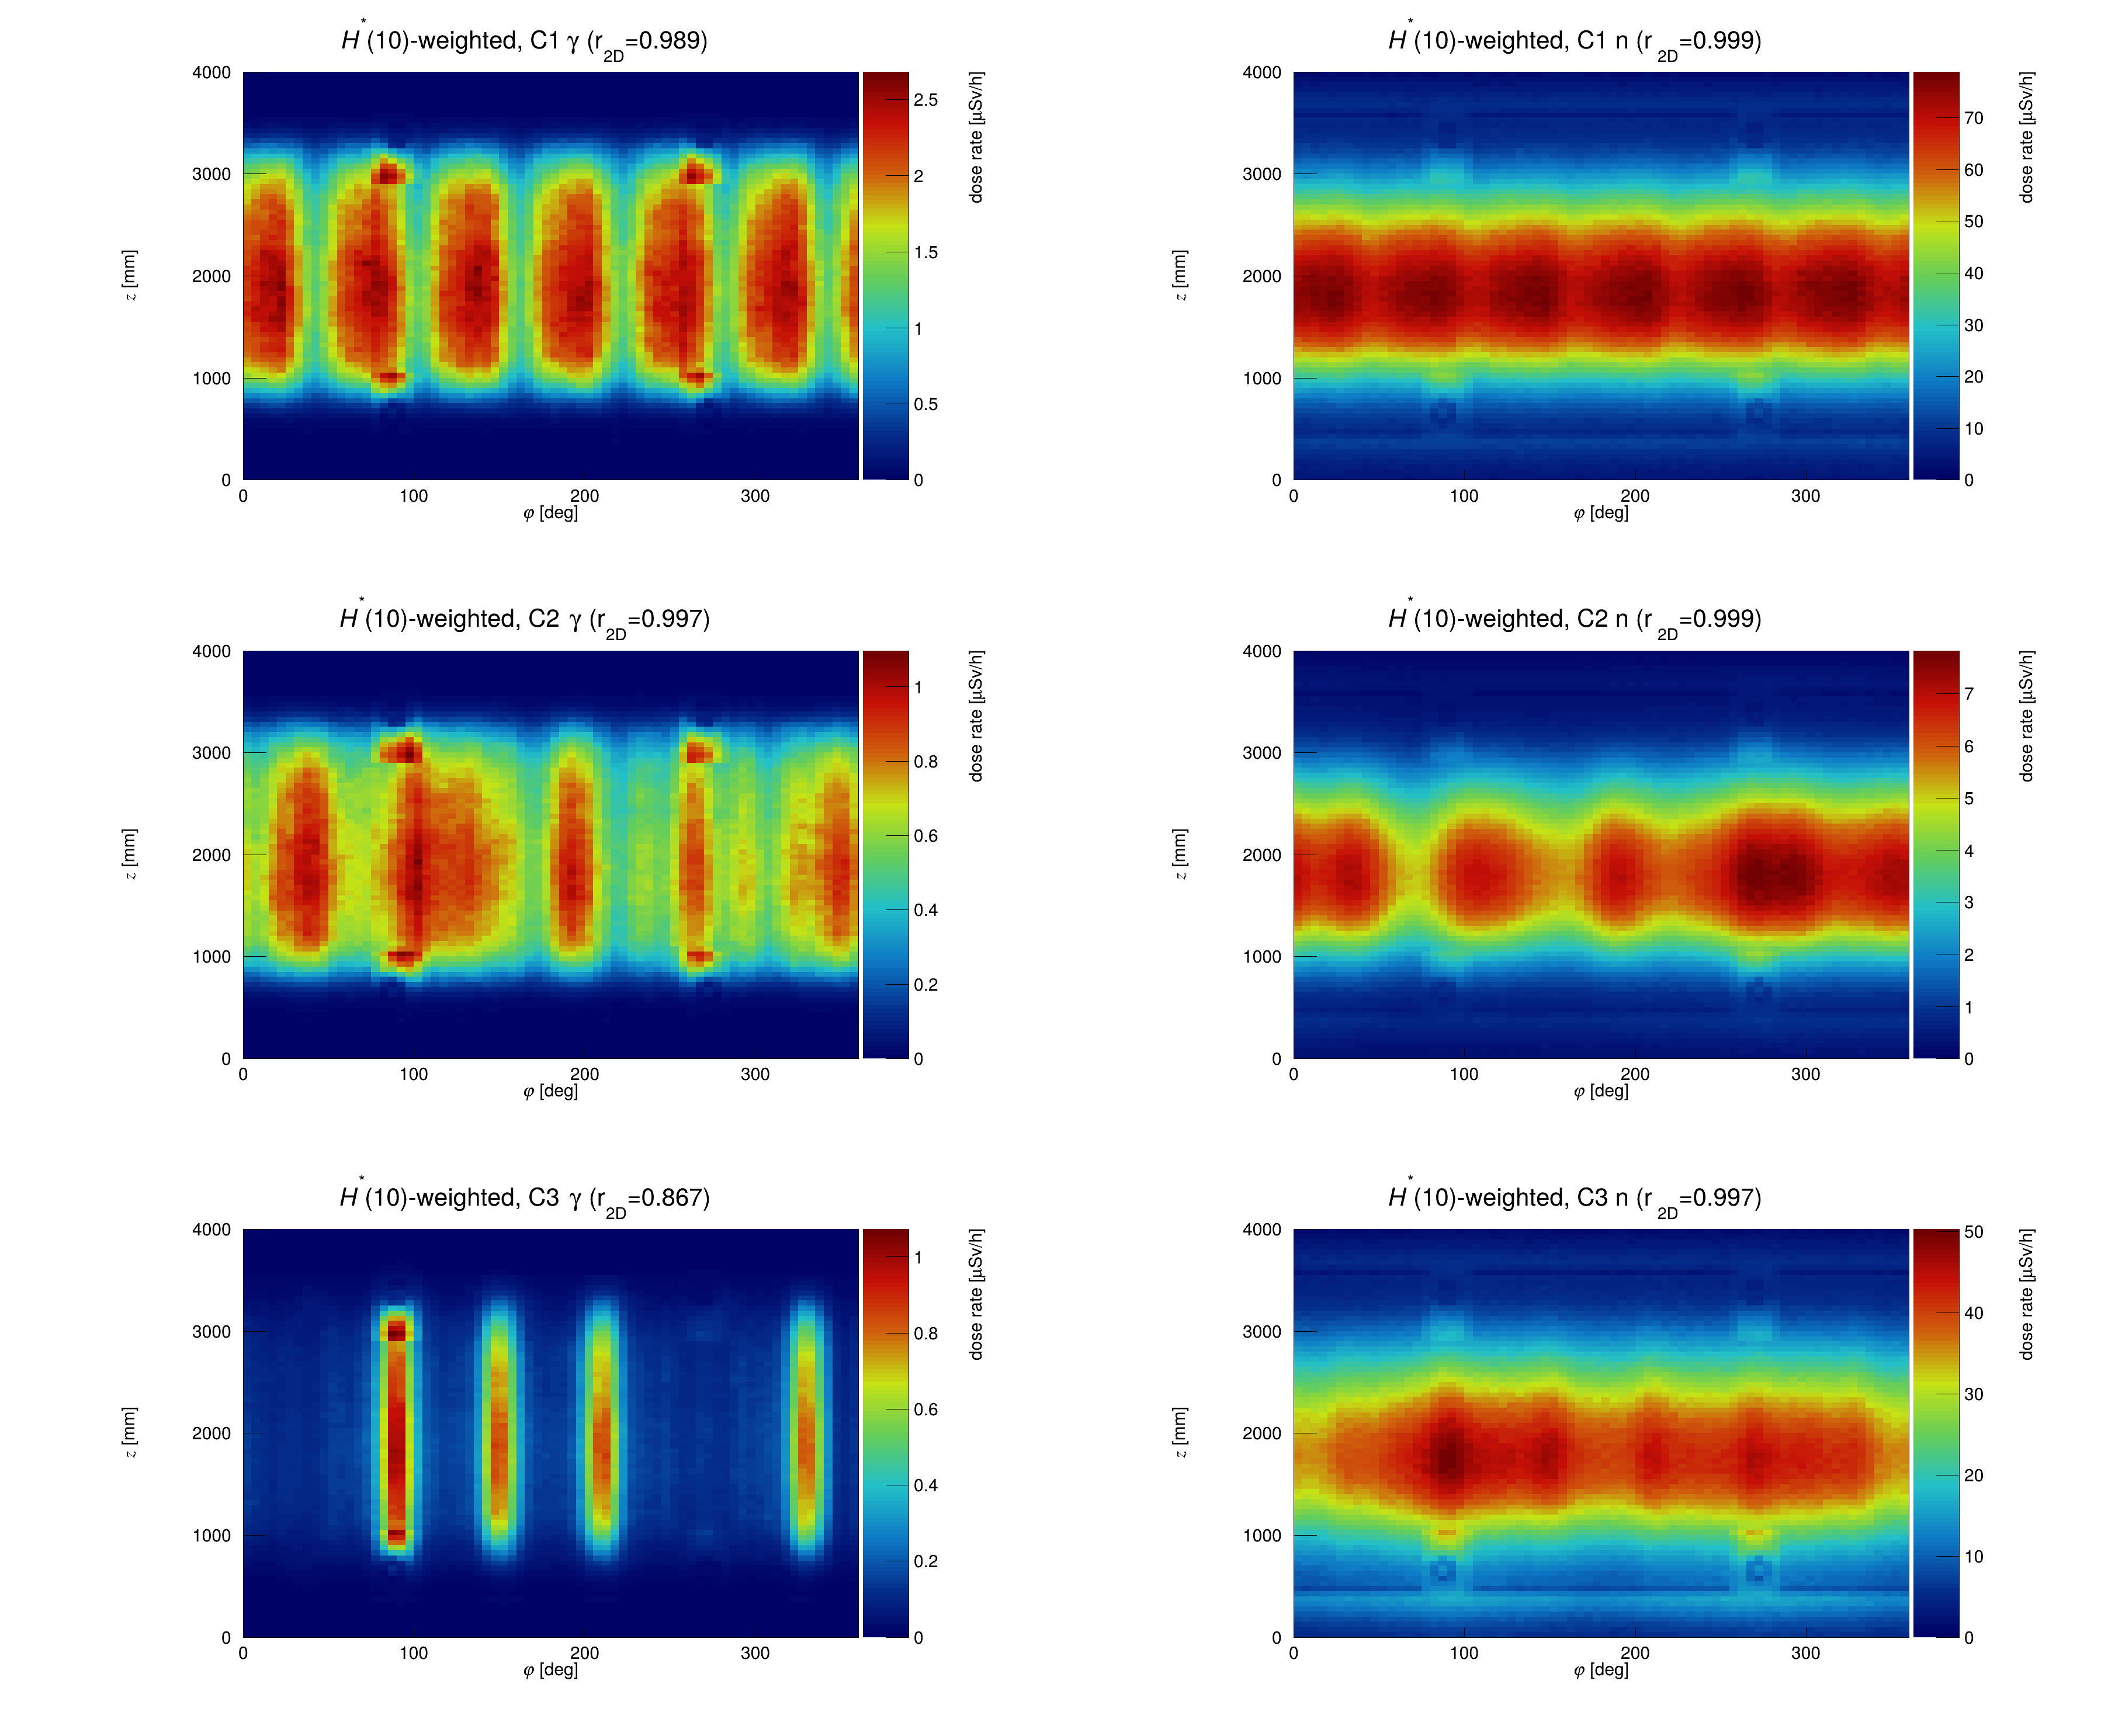
\includegraphics[width=\linewidth]{fig_data_maps_all_dose.png}
\caption{$H^*(10)$-weighted reader maps for the six WSSA files.  Rows are
Cask~1, 2, and 3 from top to bottom; columns are gamma (left) and neutrons
(right).  Each panel is the sum of $w\,H^*(10)(E)$ divided by $|np|$ and the
bin area and converted to $\mu$Sv\,h$^{-1}$ on the native 72$\times$80 grid,
with no per-maximum normalisation.  The units are the same as in the
reference PNGs; the title gives the 72$\times$80 correlation with the
digitised reference.  The maps use mode~1 (clockwise from $+y$).  The display
is per source history, not the raw sum.}
\label{fig:data_all_dose}
\end{figure}

\begin{figure}[p]
\centering
\begin{subfigure}{0.49\linewidth}
  \centering
  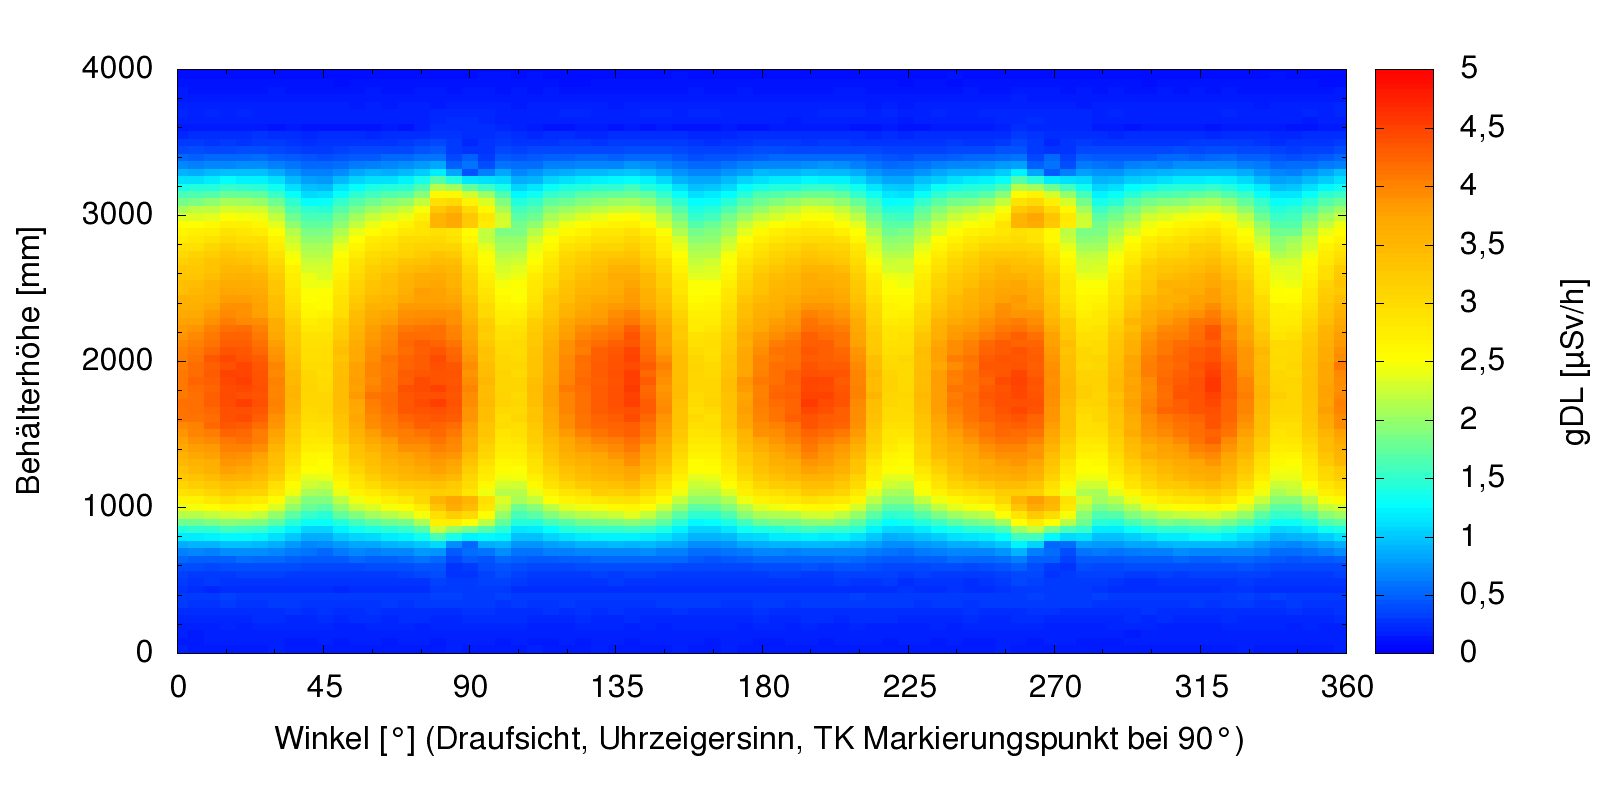
\includegraphics[width=\linewidth]{orig_Cask1_gamma.png}
  \caption{Cask~1 gamma}
\end{subfigure}
\hfill
\begin{subfigure}{0.49\linewidth}
  \centering
  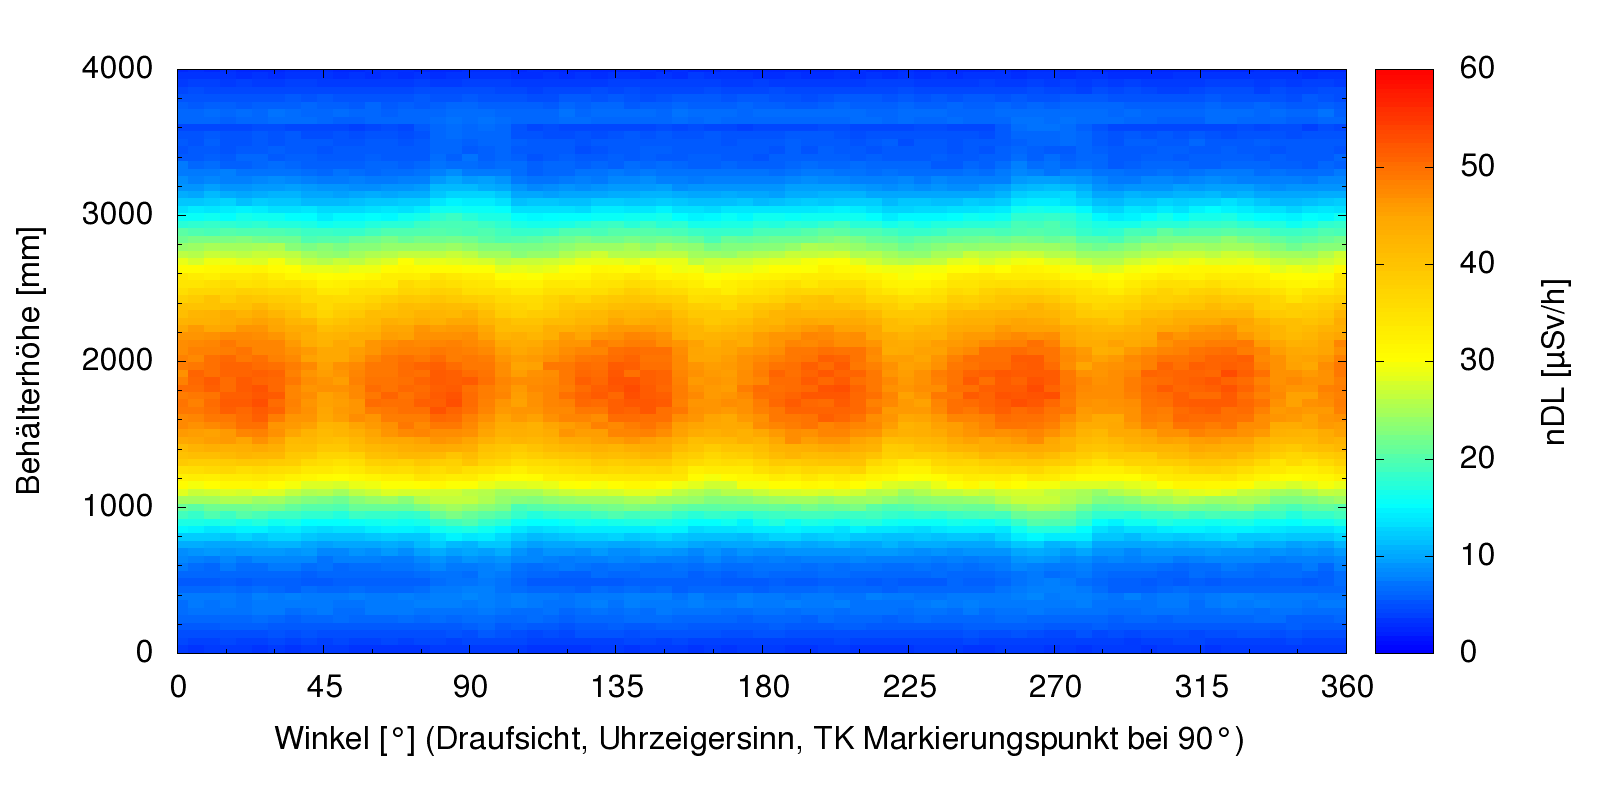
\includegraphics[width=\linewidth]{orig_Cask1_neutrons.png}
  \caption{Cask~1 neutrons}
\end{subfigure}

\vspace{0.15em}
\begin{subfigure}{0.49\linewidth}
  \centering
  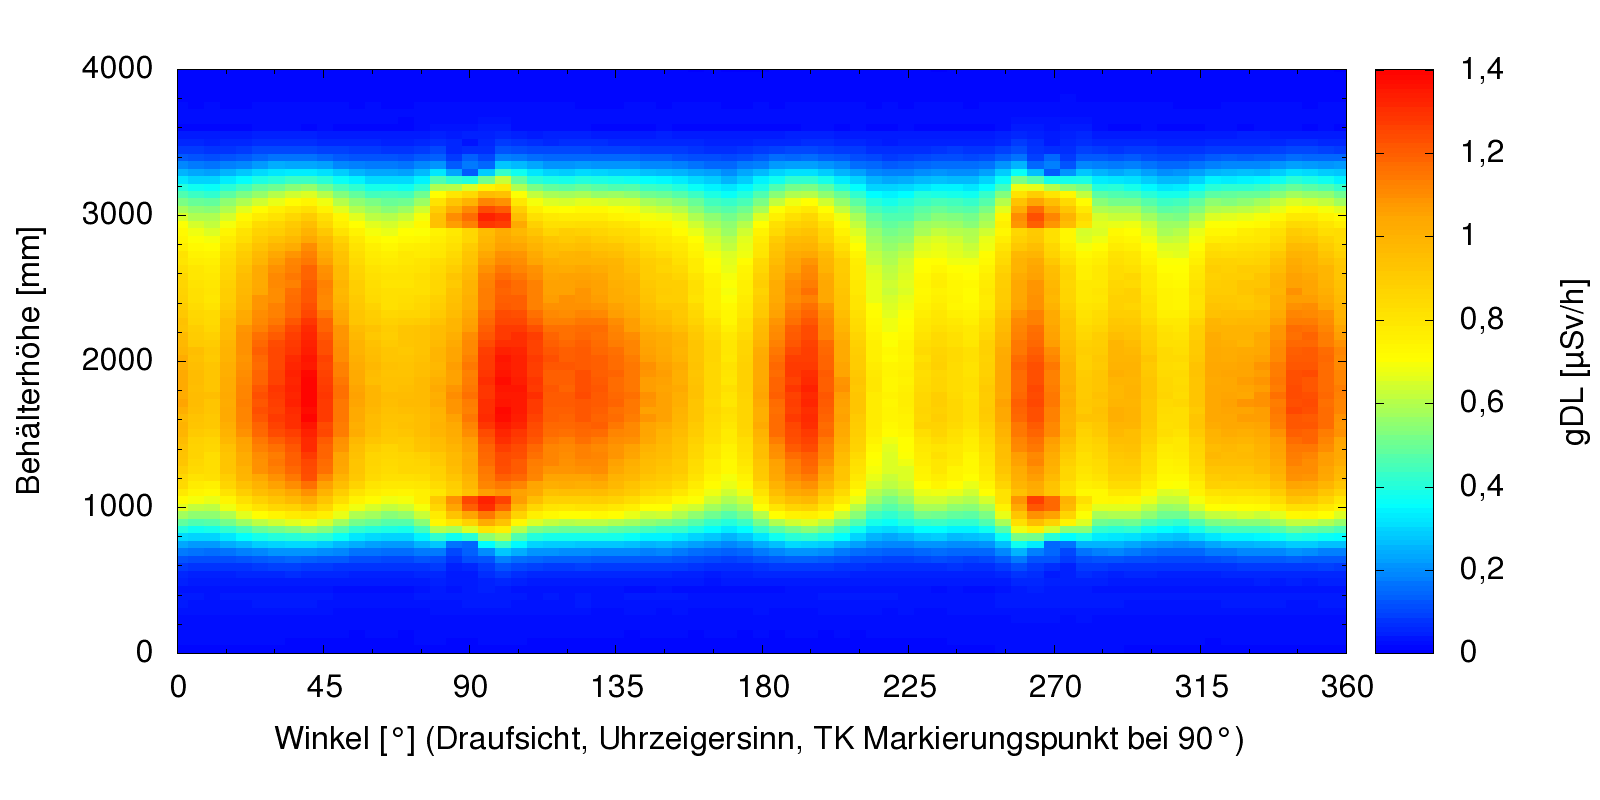
\includegraphics[width=\linewidth]{orig_Cask2_gamma.png}
  \caption{Cask~2 gamma}
\end{subfigure}
\hfill
\begin{subfigure}{0.49\linewidth}
  \centering
  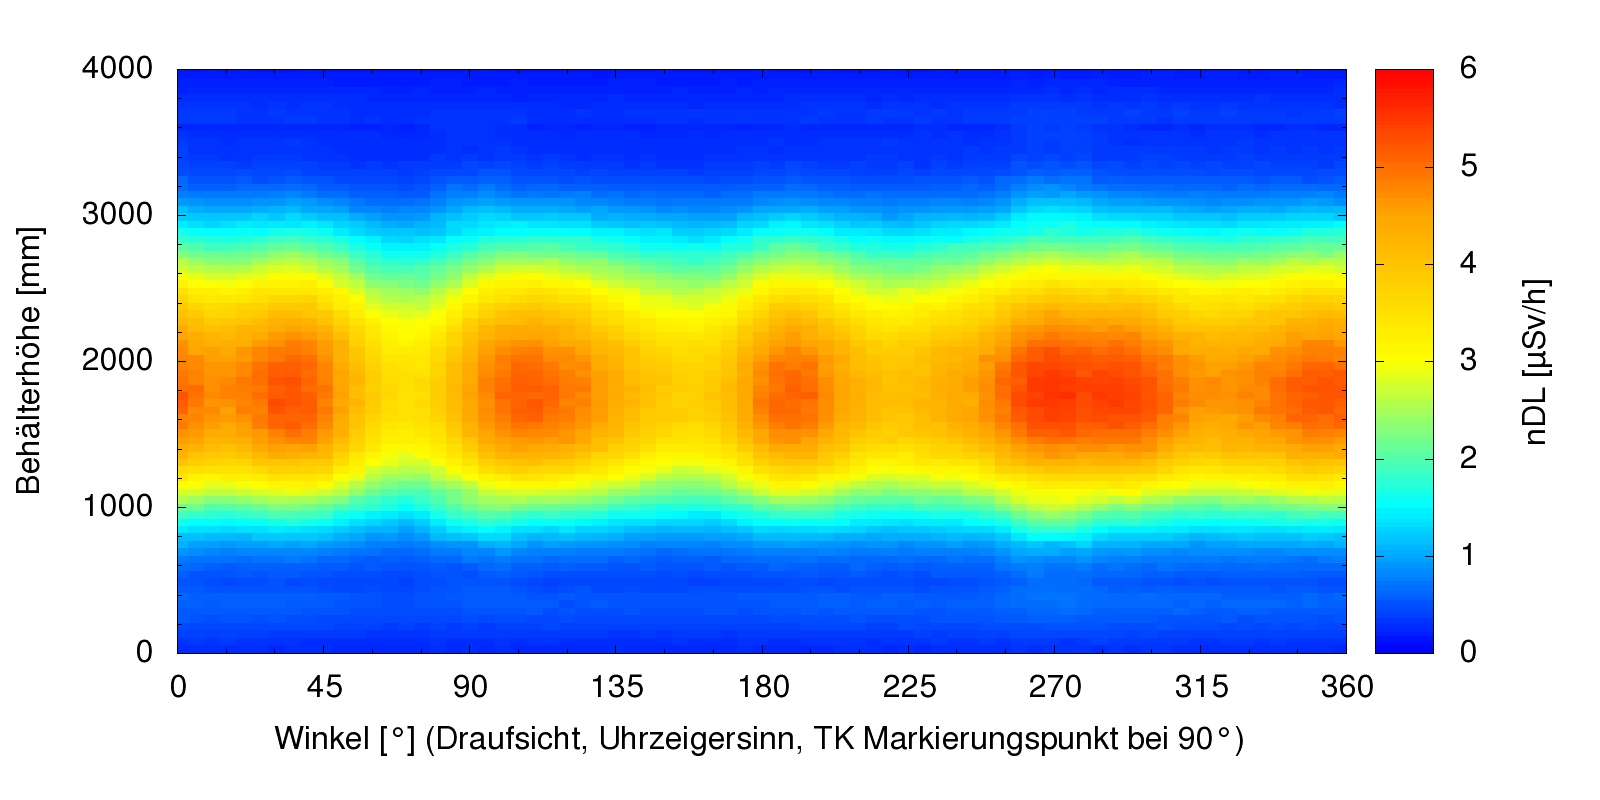
\includegraphics[width=\linewidth]{orig_Cask2_neutrons.png}
  \caption{Cask~2 neutrons}
\end{subfigure}

\vspace{0.15em}
\begin{subfigure}{0.49\linewidth}
  \centering
  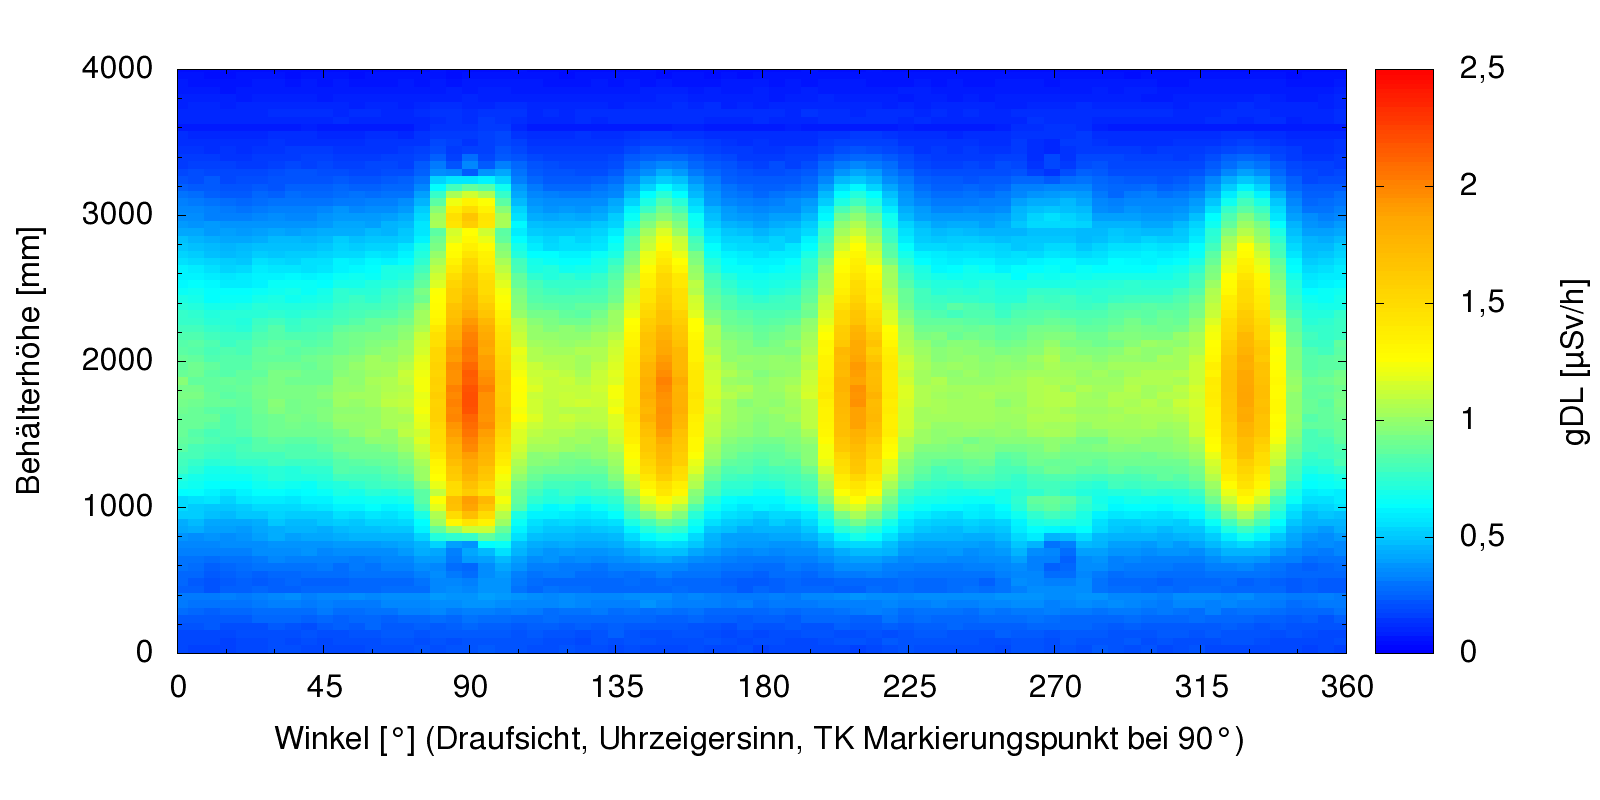
\includegraphics[width=\linewidth]{orig_Cask3_gamma.png}
  \caption{Cask~3 gamma}
\end{subfigure}
\hfill
\begin{subfigure}{0.49\linewidth}
  \centering
  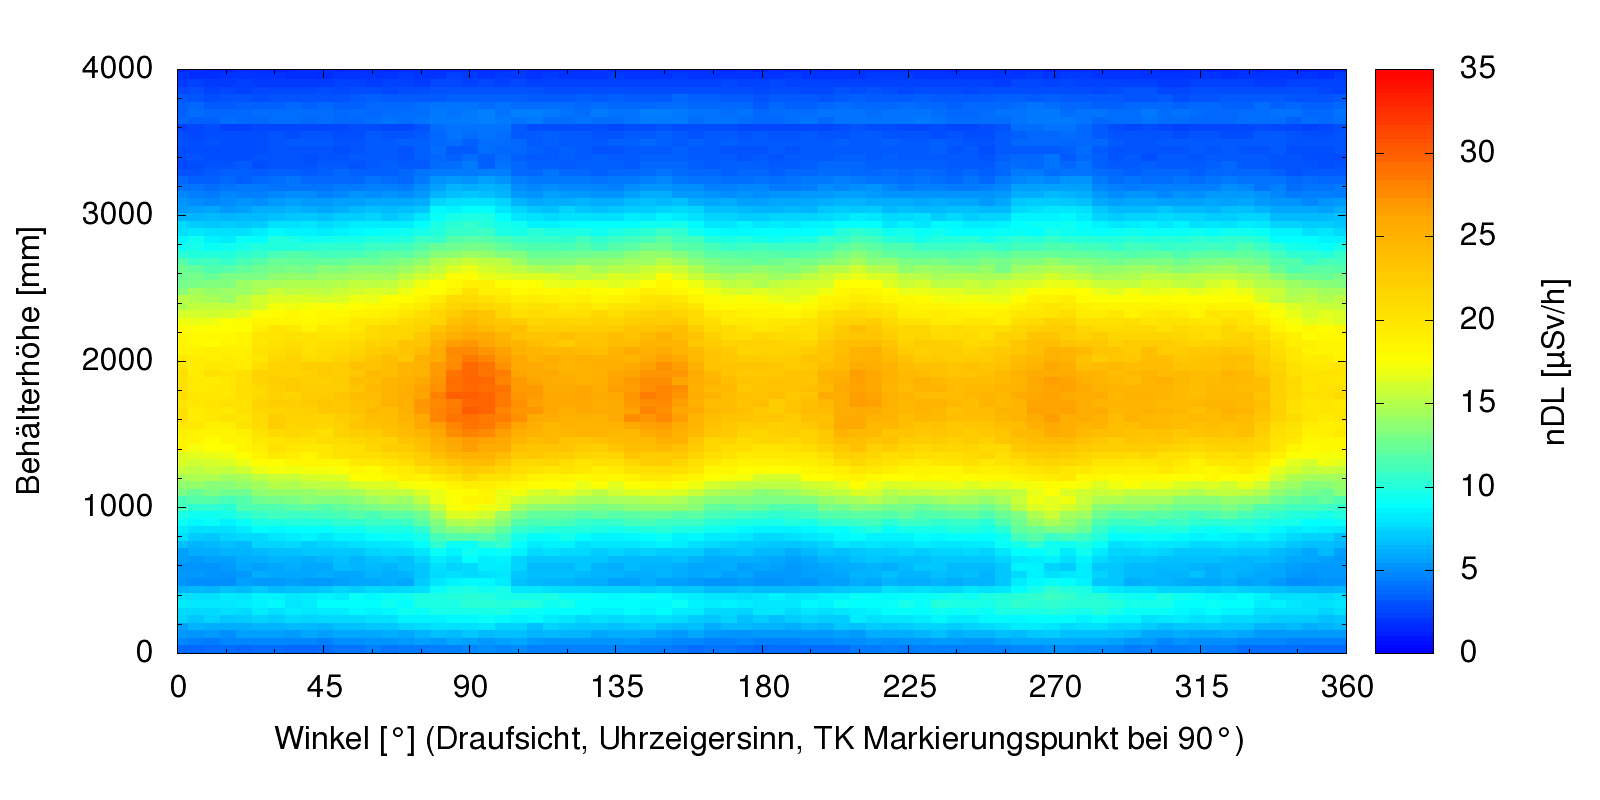
\includegraphics[width=\linewidth]{orig_Cask3_neutrons.png}
  \caption{Cask~3 neutrons}
\end{subfigure}
\caption{The six supplied reference PNGs, reproduced unchanged.  Rows are
Cask~1, 2, and 3 from top to bottom; columns are gamma (left) and neutrons
(right).  These are the source images decoded in Section~\ref{sec:part1} and
copied by the ROOT macro; the colour bars and axes are part of the supplied
image.}
\label{fig:orig}
\end{figure}

\section{Reproduction commands}\label{app:repro}

The following commands reproduce the full-file pass, the validation, and the
report figures.  Run them from the repository root unless noted.

{\small
\begin{verbatim}
# 1. Full-file pass for all six WSSA files (N=0 means every record)
root -l -b -q 'scripts/wssa/run_all_wssa.C+'

# 2. ROOT digitisation, correlations, figures, and tables
root -l -b -q 'scripts/wssa/validate_wssa_root.C+'

# 3. Absolute-scale diagnostic: six 10M sequential samples, then the CSV table
scripts/wssa/run_absolute_scale_diagnostic.sh

# 4. Report: rebuild the ROOT figures, then LaTeX
cd report/wti-binary-reader
make

# 5. Geant4 replay (from the build directory)
cd ../../build
./G4DCSmonitor run_wssa_surface.mac
\end{verbatim}
}

\begin{sloppypar}
The driver writes the six \texttt{scripts/wssa/output\_all/}\allowbreak
\texttt{<tag>\_all.root} files, each with \texttt{hPhiZ\_fine} and
\texttt{hPhiZ\_dose\_fine}, and their per-file diagnostic images.  The ROOT
macro writes \texttt{data/}\allowbreak
\texttt{full\_validation\_summary.csv} under the report directory, one
\texttt{*\_all\_validation.txt} per file, all report figures, and the copies
\texttt{figures/orig\_*.png}.  The diagnostic script writes
\texttt{scripts/wssa/output\_diag/*\_seq10m.root} and
\texttt{report/wti-binary-reader/data/absolute\_scale\_diagnostic.csv}; it uses
10M sequential records per file and the full F1 map for the F2 local-ratio
estimate.  No Python is used.  For a single file, call
\texttt{read\_wssa.C} with \texttt{N=0}, \texttt{randomMode=false},
\texttt{eMin=1e-12}, and \texttt{eMax=30}; the optional final argument selects
the dose particle (\texttt{"gamma"}, \texttt{"neutron"}, or \texttt{"auto"}),
and the coefficient table is in \texttt{scripts/wssa/ICRP74H10.hh}.
\end{sloppypar}

The template macro uses Cask~3 neutrons, a 10M cap, and a beam-on count of
1000.  Reduce the cap and the beam-on count for a quick test; set
\texttt{wssaPid} to 22 and change the file path for a gamma run.  The gamma
smoke test used a cask-only macro and 20 events.

\end{document}
